\documentclass[12pt,openany]{book}
\usepackage{lmodern}
\usepackage{setspace}
\setstretch{1.5}
\usepackage{amssymb,amsmath}
\usepackage{ifxetex,ifluatex}
\usepackage{fixltx2e} % provides \textsubscript
\ifnum 0\ifxetex 1\fi\ifluatex 1\fi=0 % if pdftex
  \usepackage[T1]{fontenc}
  \usepackage[utf8]{inputenc}
\else % if luatex or xelatex
  \ifxetex
    \usepackage{mathspec}
  \else
    \usepackage{fontspec}
  \fi
  \defaultfontfeatures{Ligatures=TeX,Scale=MatchLowercase}
\fi
% use upquote if available, for straight quotes in verbatim environments
\IfFileExists{upquote.sty}{\usepackage{upquote}}{}
% use microtype if available
\IfFileExists{microtype.sty}{%
\usepackage{microtype}
\UseMicrotypeSet[protrusion]{basicmath} % disable protrusion for tt fonts
}{}
\usepackage[left=4cm, right=3cm, top=3cm, bottom=3cm]{geometry}
\usepackage{hyperref}
\hypersetup{unicode=true,
            pdfborder={0 0 0},
            breaklinks=true}
\urlstyle{same}  % don't use monospace font for urls
\usepackage{longtable,booktabs}
\usepackage{graphicx,grffile}
\makeatletter
\def\maxwidth{\ifdim\Gin@nat@width>\linewidth\linewidth\else\Gin@nat@width\fi}
\def\maxheight{\ifdim\Gin@nat@height>\textheight\textheight\else\Gin@nat@height\fi}
\makeatother
% Scale images if necessary, so that they will not overflow the page
% margins by default, and it is still possible to overwrite the defaults
% using explicit options in \includegraphics[width, height, ...]{}
\setkeys{Gin}{width=\maxwidth,height=\maxheight,keepaspectratio}
\IfFileExists{parskip.sty}{%
\usepackage{parskip}
}{% else
\setlength{\parindent}{0pt}
\setlength{\parskip}{6pt plus 2pt minus 1pt}
}
\setlength{\emergencystretch}{3em}  % prevent overfull lines
\providecommand{\tightlist}{%
  \setlength{\itemsep}{0pt}\setlength{\parskip}{0pt}}
\setcounter{secnumdepth}{5}
% Redefines (sub)paragraphs to behave more like sections
\ifx\paragraph\undefined\else
\let\oldparagraph\paragraph
\renewcommand{\paragraph}[1]{\oldparagraph{#1}\mbox{}}
\fi
\ifx\subparagraph\undefined\else
\let\oldsubparagraph\subparagraph
\renewcommand{\subparagraph}[1]{\oldsubparagraph{#1}\mbox{}}
\fi

%%% Use protect on footnotes to avoid problems with footnotes in titles
\let\rmarkdownfootnote\footnote%
\def\footnote{\protect\rmarkdownfootnote}

%%% Change title format to be more compact
\usepackage{titling}

% Create subtitle command for use in maketitle
\newcommand{\subtitle}[1]{
  \posttitle{
    \begin{center}\large#1\end{center}
    }
}

\setlength{\droptitle}{-2em}
  \title{}
  \pretitle{\vspace{\droptitle}}
  \posttitle{}
  \author{}
  \preauthor{}\postauthor{}
  \date{}
  \predate{}\postdate{}

\usepackage[none]{hyphenat}
\usepackage[cmyk]{xcolor} % Recommended by US-AB
\usepackage{lmodern} % Recommended by US-AB
\usepackage{fancyhdr}
\usepackage{etoolbox}
\patchcmd{\chapter}{\thispagestyle{plain}}{\thispagestyle{fancy}}{}{} % Removes plain pagestyle from chapter headings (otherwise, page numbers are centered)
\AtBeginDocument{\addtocontents{toc}{\protect\thispagestyle{empty}}} 
\pagestyle{empty} % This makes ToC without header/footer
\usepackage[skip=15pt]{caption} % This should increase space below captions (not tested)
\raggedbottom

\usepackage{CJKutf8} % For Mandarin in Acknowledgments

% For guiding quote in beginning of intro:
\makeatletter
% \renewcommand{\@chapapp}{}% Not necessary...
\newenvironment{chapquote}[2][2em]
  {\setlength{\@tempdima}{#1}%
   \def\chapquote@author{#2}%
   \parshape 1 \@tempdima \dimexpr\textwidth-2\@tempdima\relax%
   \itshape}
  {\par\normalfont\hfill--\ \chapquote@author\hspace*{\@tempdima}\par\bigskip}
\makeatother

\usepackage{amsthm}
\newtheorem{theorem}{Theorem}[chapter]
\newtheorem{lemma}{Lemma}[chapter]
\theoremstyle{definition}
\newtheorem{definition}{Definition}[chapter]
\newtheorem{corollary}{Corollary}[chapter]
\newtheorem{proposition}{Proposition}[chapter]
\theoremstyle{definition}
\newtheorem{example}{Example}[chapter]
\theoremstyle{definition}
\newtheorem{exercise}{Exercise}[chapter]
\theoremstyle{remark}
\newtheorem*{remark}{Remark}
\newtheorem*{solution}{Solution}
\begin{document}

{
\setcounter{tocdepth}{1}
\tableofcontents
}
\cleardoublepage

\pagestyle{fancy} \fancyhf{} \renewcommand{\headrulewidth}{0pt}
\fancyfoot[LE,RO]{\thepage} \renewcommand{\floatpagefraction}{.9}

\setcounter{page}{9}

\chapter*{Abbreviations}\label{abbreviations}
\addcontentsline{toc}{chapter}{Abbreviations}

\begin{tabular}{ll}
\toprule
Abbreviation & Term\\
\midrule
ACC & Anterior Cingulate Cortex\\
BOLD & Blood Oxygen Level Dependent\\
DDM & Drift Diffusion Model\\
fMRI & Functional Magnetic Resonance Imaging\\
MRI & Magnetic Resonance Imaging\\
PES & Post-Error Slowing\\
pMFC & Posterior Medial Frontal Cortex\\
PFC & Prefrontal Cortex\\
pre-SMA & Presupplementary Motor Area\\
RT & Reaction Time\\
ROI & Region Of Interest\\
RL & Reinforcement Learning\\
rIFC & Right Inferior Frontal Cortex\\
rIFG & Right Inferior Frontal Gyrus\\
SSRT & Stop Signal Reaction Time\\
STN & Subthalamic Nucleus\\
2AFC & Two-Alternative Forced Choice\\
\bottomrule
\end{tabular}

\chapter{Introduction}\label{introduction}

\begin{chapquote}{William James, \textit{Principles of Psychology}}
One of the lines of experimental investigation most diligently followed of late years is that of the ascertainment of the time occupied by nervous events. [...] The question is, What happens inside of us, either in brain or in mind? and to answer that we must analyze just what processes the reaction involves.
\end{chapquote}

\section{Conceptual overview}\label{conceptual-overview}

Both on the behavioural and neural level tremendous progress has been
made over the past decades in the understanding of how stimulus values
lead to action and how actions can be constrained by exerting cognitive
control over them. However, these two processes of reinforcement
learning and cognitive control have predominantly been investigated in
isolation, particularly in neuroscience. Therefore, the question of how
appropriate behavioural adjustment according to feedback improves value
learning has only recently come into the spotlight. This question will
stand in the center of this thesis.

I will start by providing separate overviews of the fields of cognitive
control and reinforcement learning and afterwards I am going to
highlight interactions between the two fields, particularly in the realm
of mental disorders.

\section{Cognitive control}\label{cognitive-control}

Cognitive control refers to a heterogeneous concept, subsuming a variety
of mental functions which include, but are not limited to, working
memory, task-set switching, response selection and response inhibition
(Lenartowicz, Kalar, Congdon, \& Poldrack, 2010; Ridderinkhof,
Wildenberg, Segalowitz, \& Carter, 2004; Sabb et al., 2008; Ullsperger,
Danielmeier, \& Jocham, 2014). As a whole it can be defined as ``the
ability to regulate, coordinate, and sequence thoughts and actions in
accordance with internally maintained behavioral goals'' (Braver, 2012).
In this thesis I will mainly focus on behavioural and neural aspects of
response inhibition in order to implement adaptive behaviour.

\subsection{Post-error slowing (PES)}\label{post-error-slowing-pes}

An example of response inhibition is the phenomenon of post-error
slowing (PES). After making a mistake or receiving negative feedback in
a task, the next response on similar trials will often require a longer
reaction time than pre-error responses (Danielmeier \& Ullsperger, 2011;
Kerns et al., 2004).

Various accounts have been proposed to explain the psychological
correlates to this slowing. On the one hand, non-functional accounts of
PES contend that the slowing happens because of the low frequency of
errors in many tasks which evokes a general orienting response
(Notebaert et al., 2009) or that post-error monitoring acts as a
bottleneck, limiting resources of decision processes after the error
(Jentzsch \& Dudschig, 2009). A common motive among the functional
accounts of PES on the other hand is to argue for an increase in
response caution (Botvinick, Braver, Barch, Carter, \& Cohen, 2001;
Dutilh et al., 2012b) on the trial following the error which leads to a
speed-accuracy trade-off (Bogacz, Wagenmakers, Forstmann, \&
Nieuwenhuis, 2010; Fitts, 1966; Heitz, 2014; Laming, 1979; Steinhauser,
Ernst, \& Ibald, 2017).

PES is often quantified in response time tasks such as Go/No-Go tasks,
where the response time after an error is subtracted from the response
time on the trial before the error (Dutilh et al., 2012a). Similarly, it
can be calculated in relation to a comparable previous trial, even if
that trial is set apart in time by several seconds (Cavanagh, Frank,
Klein, \& Allen, 2010; Frank, Moustafa, Haughey, Curran, \& Hutchison,
2007). While the former might reflect a motoric or more general
attentional adjustment, the latter also takes into account the
adaptation of response speed in accordance to conflict between two
stimuli with similar values.

For example, in a probabilistic reinforcement learning task such as we
have employed in \textbf{Study I} and \textbf{II}, negative feedback
should trigger response speed decreases the next time a particular
symbol pair is seen, which would show an adaptive regulation of response
time in accordance with feedback (Figure \ref{fig_pes}A). This response
time slowing could be useful to gather more evidence when stimulus
values are more similar to each other and therefore harder to
distinguish, i.e., during conflict (Cavanagh et al., 2011; Frank et al.,
2015; Zaghloul et al., 2012). On the other hand, errors on a visual
search task such as the one we used in \textbf{Study III} might be
expected to have the largest effect on trials directly after the error
since the task is structured deterministically and errors provide
information about necessary adaptation on the immediate next trial
(e.g., ``I missed this angry face, therefore I need to check for this
particular face shape more carefully'', see Figure \ref{fig_pes}B).

\begin{figure}
\centering
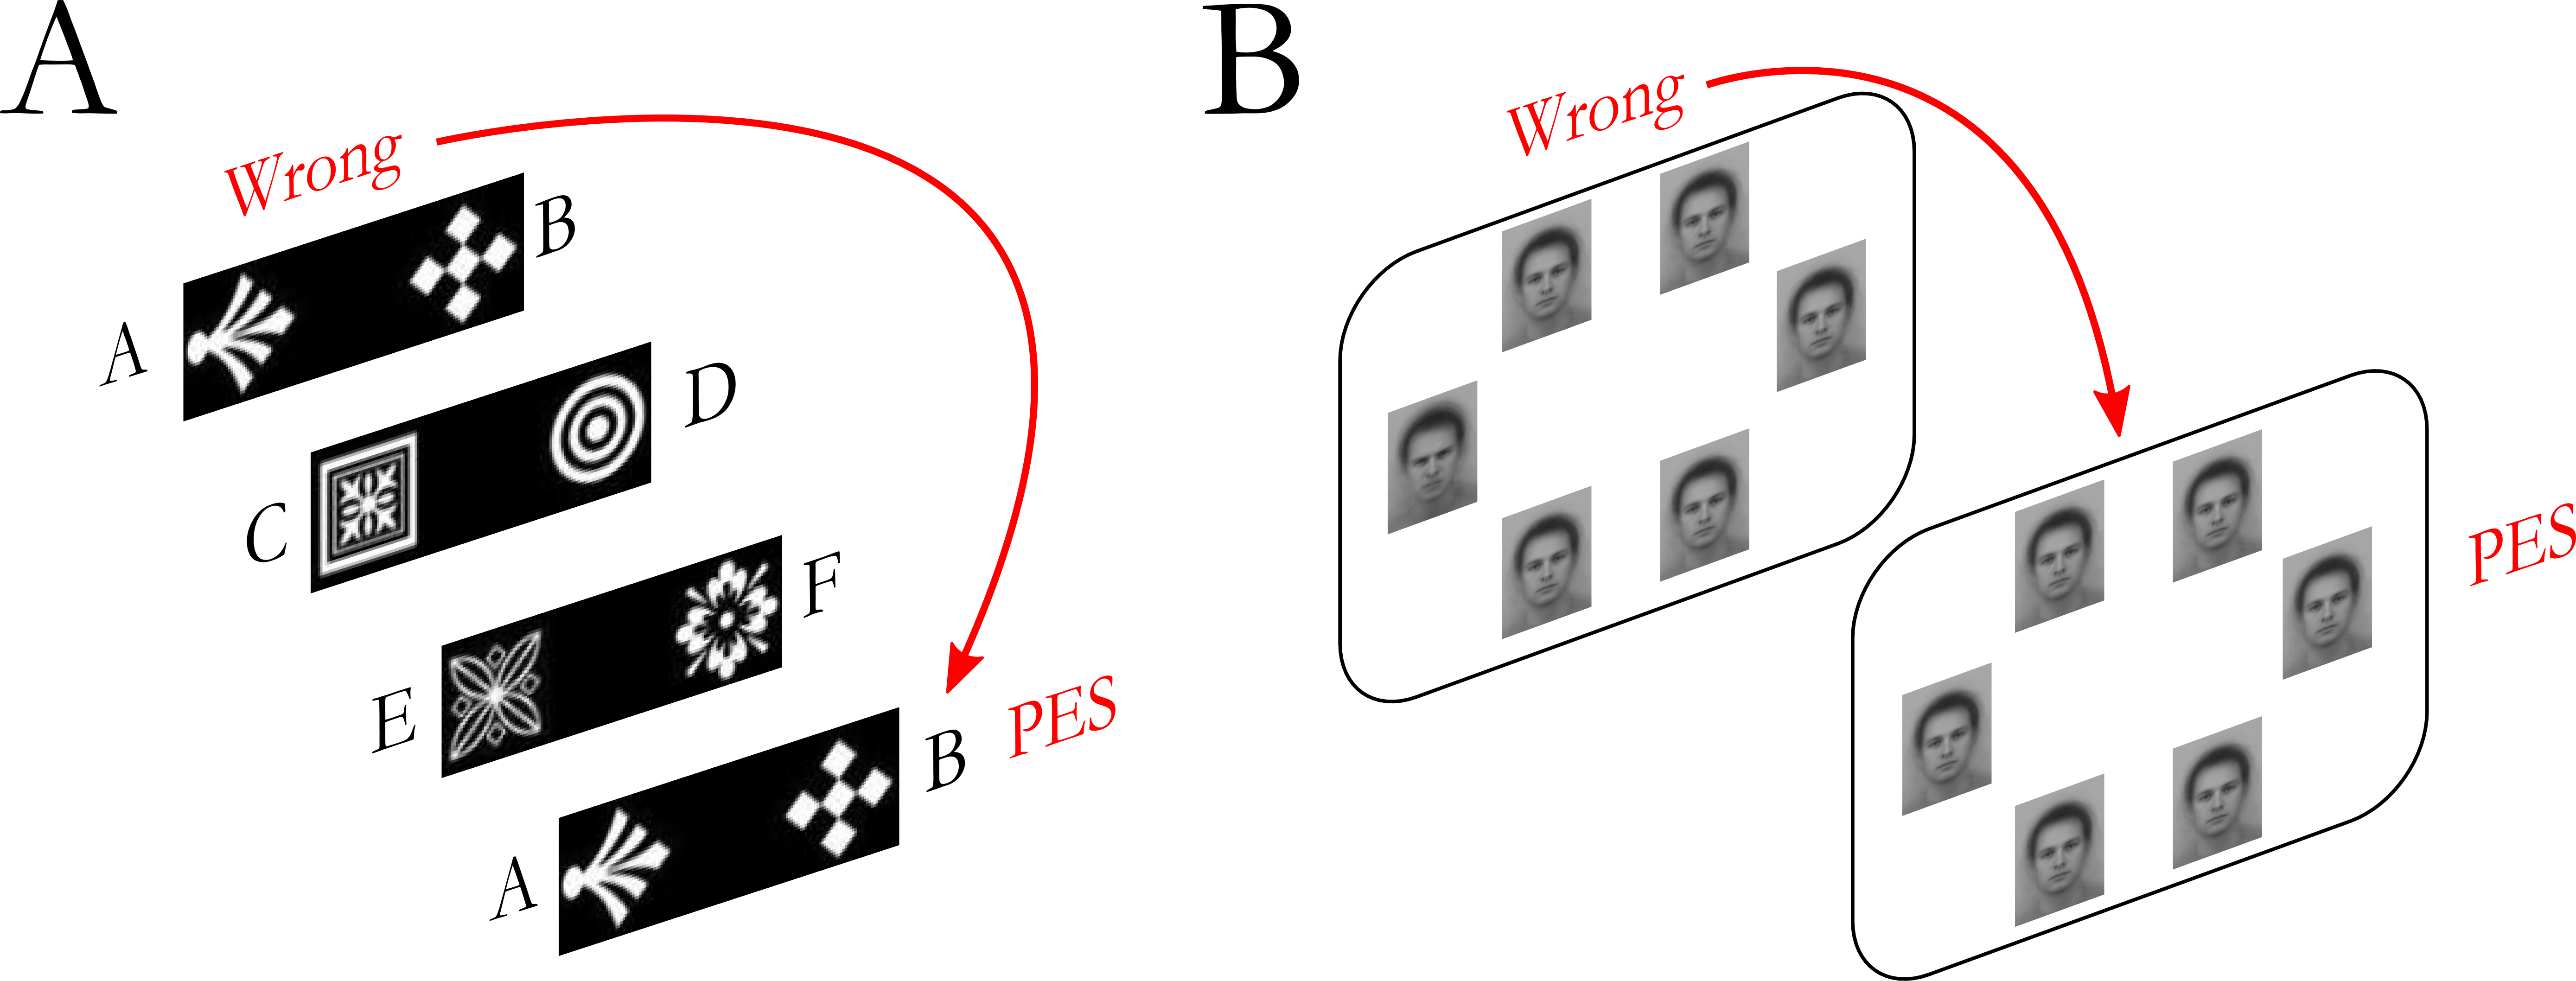
\includegraphics{./figures/pes_memory_direct.png}
\caption{The two different kinds of post-error slowing investigated in
this thesis. (A) PES during a probabilistic reinforcement learning task
as employed in our \textbf{Studies I} and \textbf{II}. Here, PES
(\(\Delta\)RT) is calculated by subtracting the RT on the error trial
from the RT when the same pair trial next appears again. (B) PES during
a visual search task as used in our \textbf{Study III}. In this study,
\(\Delta\)RT is calculated by subtracting the RT on the trial after the
error from the RT on the trial before the error if both trial conditions
are the same (in this case all neutral faces).\label{fig_pes}}
\end{figure}

\subsection{The cognitive control network in the
brain}\label{the-cognitive-control-network-in-the-brain}

Cognitive control processes are implicated to rely on lateral prefrontal
brain areas (see e.g., the review by Miller, 2000) and anterior
cingulate cortex as indicated in a lesion mapping review with a variety
of neuropsychological tasks related to response inhibition, conflict
monitoring and switching (Gläscher et al., 2012). A particular network
that implements response inhibition or stopping depending on the task at
hand has been proposed by Aron and colleagues (Figure
\ref{fig_rifg_dcm}A, Aron, Behrens, Smith, Frank, \& Poldrack, 2007;
Aron, Robbins, \& Poldrack, 2014). Within this network, right inferior
frontal gyrus (rIFG) plays a key role in response inhibition via its
connections to basal ganglia (subthalamic nucleus, STN) and
presupplementary motor area (pre-SMA). Anatomical connections between
the areas in this cognitive control network show good test-retest
reliability as assessed in a recent diffusion weighted imaging study
(Boekel, Forstmann, \& Keuken, 2017).

PES has been linked to posterior medial frontal cortex (pMFC) activity,
increased activity in task-relevant areas and decreased activity in
task-irrelevant cortical areas (Danielmeier, Eichele, Forstmann,
Tittgemeyer, \& Ullsperger, 2011; J. A. King, Korb, Cramon, \&
Ullsperger, 2010). The interesting dynamic here is that higher activity
in pMFC after feedback was correlated with an increase in PES on the
post-error trial (Danielmeier et al., 2011) while decreases in motor
network activity on the post-error trial were related to a decrease in
PES (J. A. King et al., 2010).

A recent study combining effective and anatomical connectivity methods
(Dynamic Causal Modelling and diffusion based probabilistic
tractography) showed that the rIFG positively modulates the excitatory
influence of the pre-SMA on the STN, leading to stronger motor
inhibition in motor cortex (Figure \ref{fig_rifg_dcm}B, Rae, Hughes,
Anderson, \& Rowe, 2015). Importantly, mean diffusivity in white matter
tracts connecting rIFG and preSMA to STN correlated with better
performance in inhibiting responses in a stop-signal task.

\begin{figure}
\centering
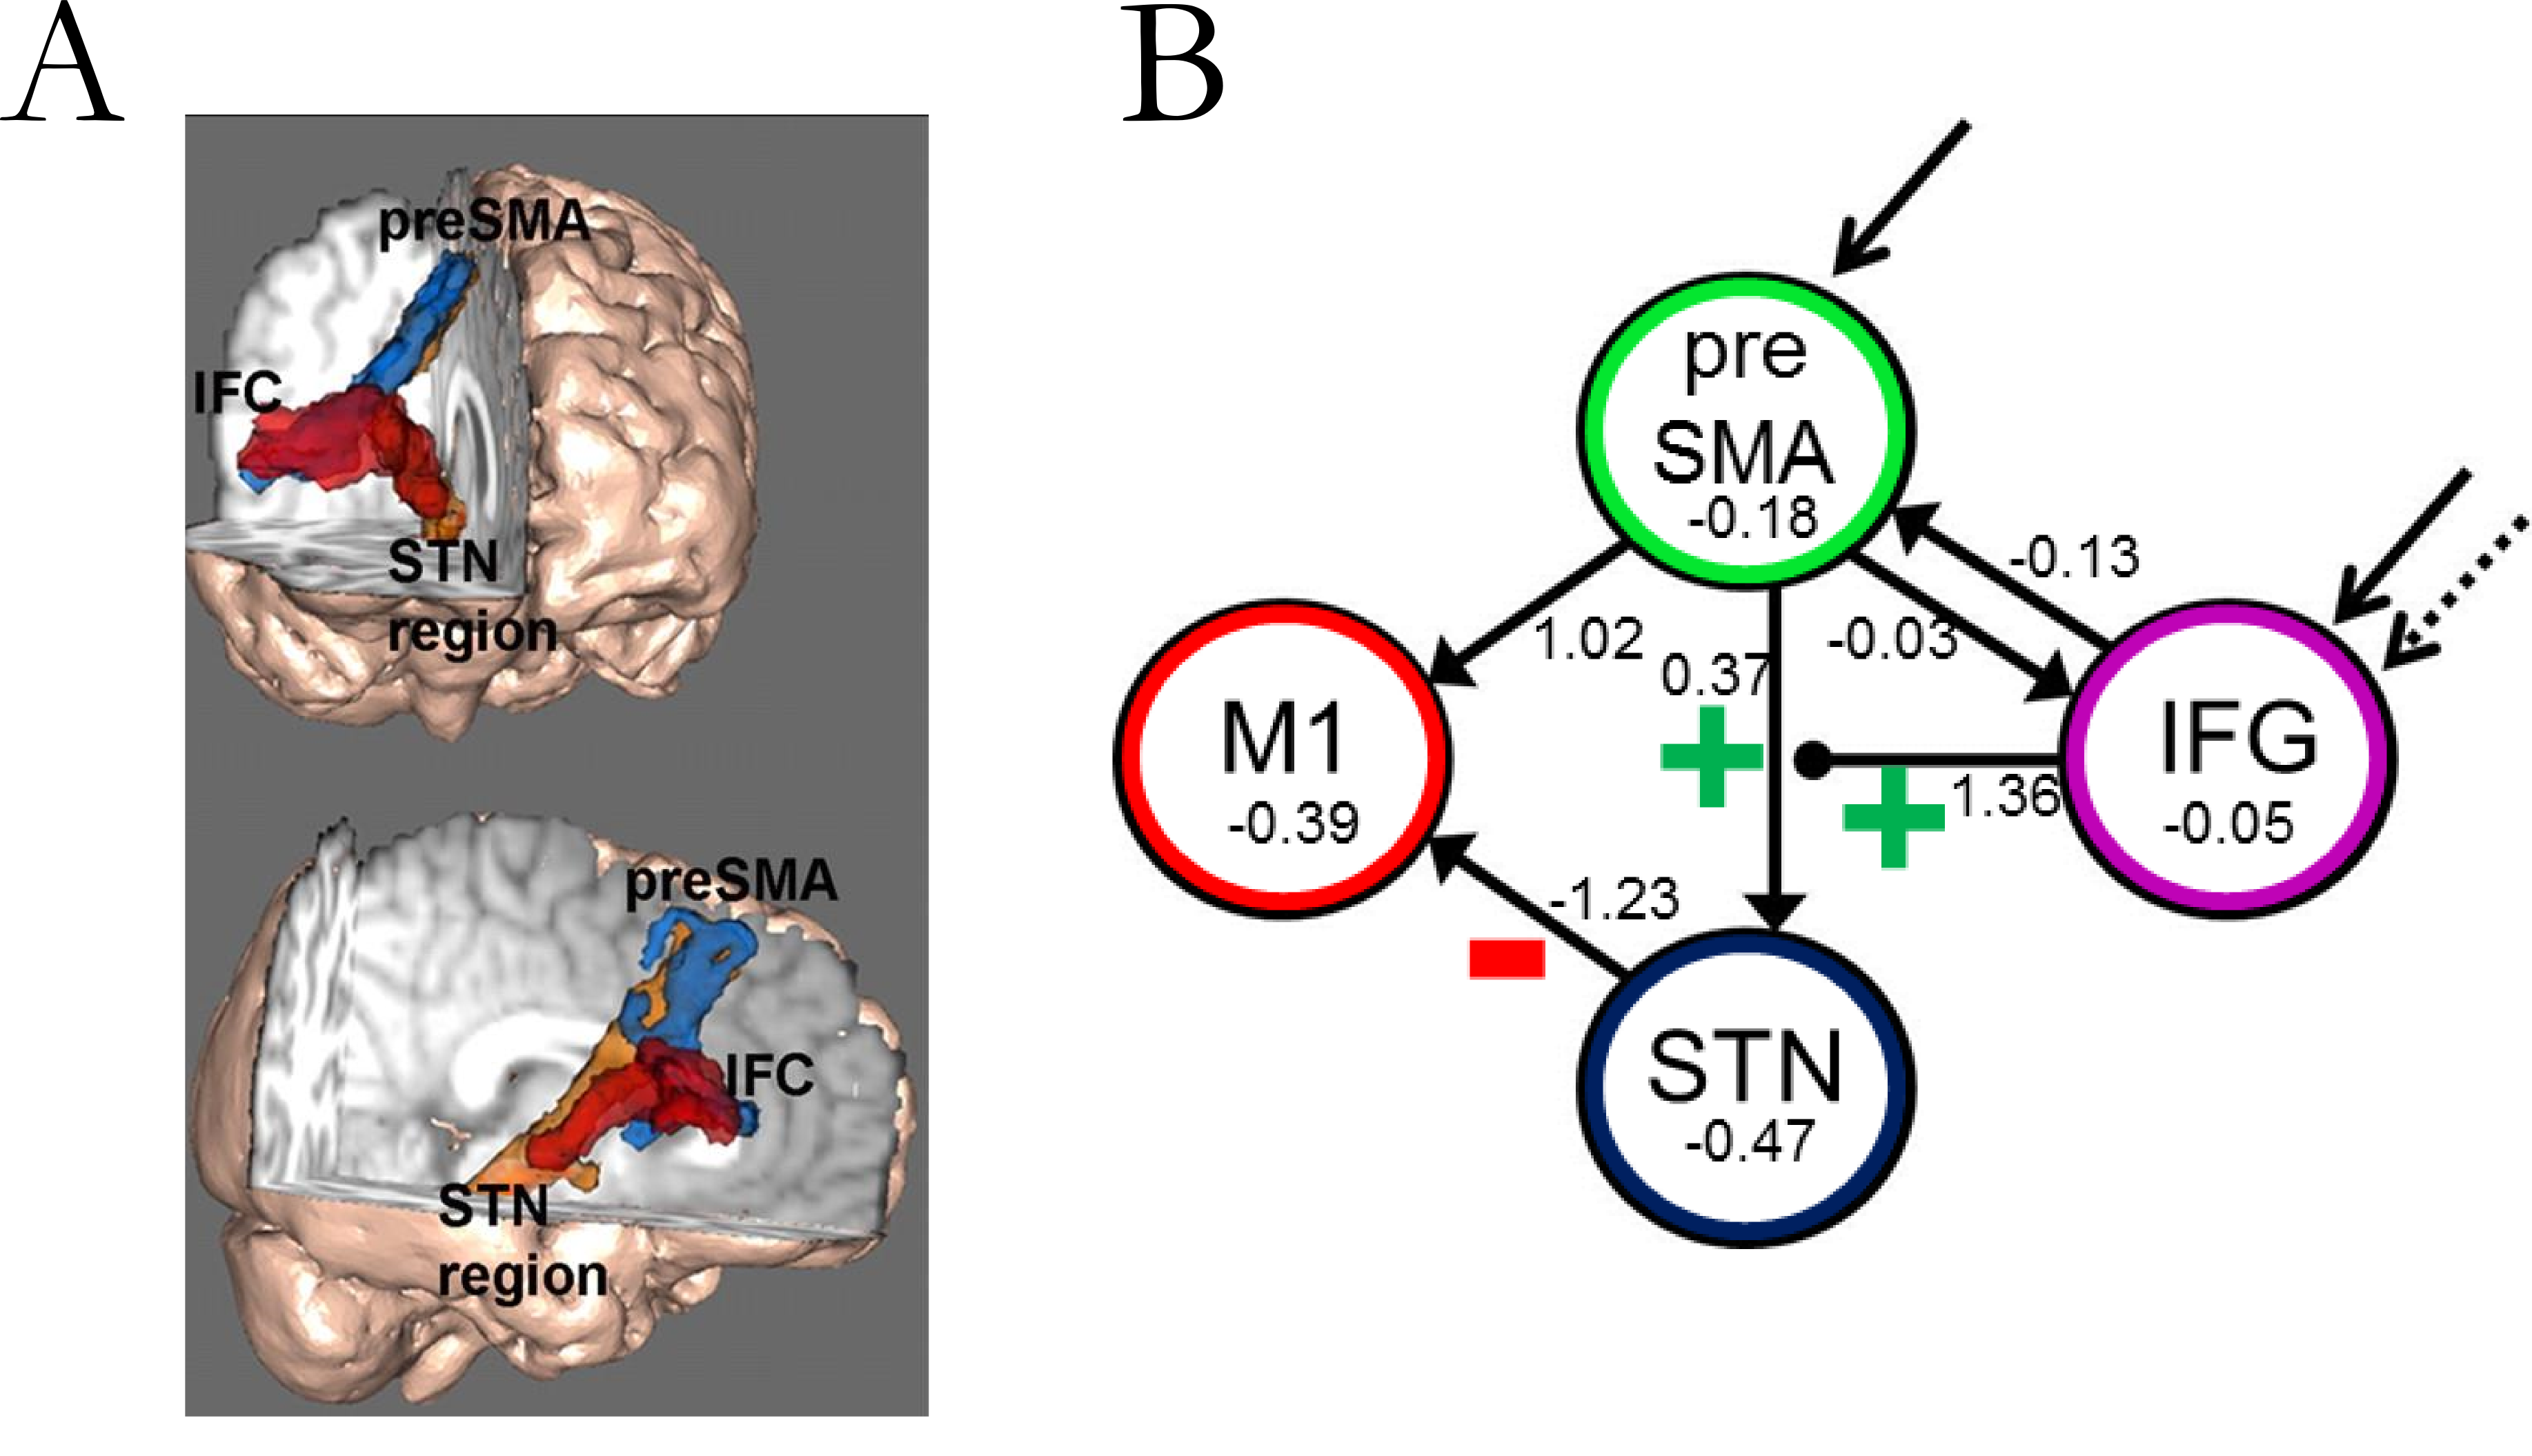
\includegraphics{./figures/dcm.png}
\caption{Major nodes of a prefrontal cognitive control network. (A)
White matter tracts connecting the right IFC, preSMA and STN are
visualized using Diffusion Weighted Imaging. Figure from Aron et al.
(2007), reprinted with permission from Society for Neuroscience. (B)
Dynamic Causal Modelling of the cognitive control network. The winning
model configuration suggests a modulating influence of IFG on the
activity between preSMA and STN. Figure from Rae et al. (2015),
reprinted under CC BY 4.0 license.\label{fig_rifg_dcm}}
\end{figure}

Extent of lesion damage to rIFG has previously been found to correlate
with a classical measure of response inhibition, the stop signal
reaction time (SSRT) in a stop signal task (Aron, Fletcher, Bullmore,
Sahakian, \& Robbins, 2003) and temporary deactivation of the rIFG using
transcranial magnetic stimulation lead to the inability of stopping an
action (Chambers et al., 2006).

Further, studies have shown that white matter integrity connecting the
rIFG and other areas relevant for cognitive control showed an
association to response inhibition performance (Fjell, Westlye, Amlien,
\& Walhovd, 2012; Madsen et al., 2010).

Based on these results of a crucial role of rIFG in response inhibition,
in \textbf{Study II} we therefore evaluated the hypothesis whether
cortical thickness in rIFG could be related to decision components
involved in post-error slowing.

\section{Reinforcement learning}\label{reinforcement-learning}

One of the largest influences on modern approaches to reinforcement
learning are behavioural studies in animals, carried out at the
beginning of the last century. In the framework of classical
conditioning, Pavlov used the term ``reinforcement'' as the repeated
pairing between an unconditioned (e.g., food) and a neutral stimulus
(e.g., a bell) until the neutral stimulus by itself led to the response
(e.g., dogs' salivation) previously only associated with the
unconditioned stimulus (Pavlov, 1927). Thus, reinforcement here refers
to an association between two stimuli.

Thorndike on the other hand specified an action-stimulus association in
his Law of Effect, derived from seminal experiments with cats
(Thorndike, 1911). This law pertains to the observation that behaviour
that is followed by positive consequences is likely going to be repeated
in the future, e.g., a cat pressing a lever to escape a box and obtain
the fish outside the box, a process later on referred to as instrumental
or operant conditioning (Skinner, 1935). Modern computational approaches
to reinforcement learning implement both Pavlovian and instrumental
conditioning to model behaviour by utilizing algorithms from the field
of machine learning (Sutton \& Barto, 1998).

A highly influential model depicting Pavlovian conditioning in animals
was developed by Rescorla \& Wagner (1972). This model was particularly
popular as it could explain key behavioural findings in reinforcement
learning such as blocking (Niv, 2009). Blocking refers to the finding
that a second conditioned stimulus does not evoke a conditioned response
if it does not provide additional information beyond that of the first
conditioned stimulus (Kamin, 1969).

Sutton and Barto (Sutton, 1988; Sutton \& Barto, 1990) extended these
ideas with the concept of temporal difference learning, incorporating
future rewards, discounted by how far they were set apart in time. This
can be a useful property when trying to explain processes like
second-order conditioning and conditioned reinforcement (Niv \&
Schoenbaum, 2008). In second-order conditioning, a stimulus that had
previously been conditioned can then be associated with another stimulus
to construct a chain of associations. For example, an animal which has
learned to associate the ringing of a bell with food can be taught to
associate a light with the bell alone and through those contingencies
learn a higher-order association between light and food. Temporal
difference learning has been successfully applied to describe this type
of second-order conditioning in humans (Seymour et al., 2004).

Here, the notion of a prediction error was also introduced, indicating
the calculation of a predicted reward minus the actual obtained reward.
I will refer back to the prediction error, particularly in terms of
reward learning, in the section on neural correlates of reinforcement
learning.

Actions that lead to rewards are subsequently repeated. This is taken
into account in Q-learning models (Watkins, 1989; Watkins \& Dayan,
1992). Here, state-action pairs, instead of state-value pairs, are
modelled as Q-values with the ``best'' actions referring to the ones
with the highest Q-values (Niv, 2009). The estimated values can then
also be used to calculate a prediction error. The SARSA
(state-action-reward-state-action) algorithm on the other hand is
considered an on-policy algorithm, meaning that the calculation of the
prediction error only involves the next chosen action, i.e., following
the agent's policy (Niv, 2009). In recent years, both using Q-learning
(e.g., FitzGerald, Friston, \& Dolan, 2012; Frank et al., 2007) and
SARSA (e.g., Daw, 2011; Gläscher, Daw, Dayan, \& O'Doherty, 2010)
algorithms to model human behaviour have proved to be useful and
reinforcement learning approaches have also improved performance of
artificial intelligence algorithms such as deep learning to match or
improve upon human performance (Mnih et al., 2015; Silver et al., 2017).

Furthermore, a division between model-free and model-based reinforcement
learning has also been proposed. While the former refers to the simple
storing of action-value correspondences without assuming a causal
structure of the environment, the latter emphasizes that decisions which
lead to rewards are made through planning and simulating the potential
actions in a goal-directed manner (Botvinick \& Weinstein, 2014).
Whether these two different systems are also dissociable in terms of
their neural correlates is still being discussed, see e.g., Daw (2011)
for evidence in favour of an integrated system, Gläscher et al. (2010)
and Smittenaar, FitzGerald, Romei, Wright, \& Dolan (2013) for accounts
of separable neural regions, S. W. Lee, Shimojo, \& O'Doherty (2014) for
an arbitration mechanism between the two systems, as well as Wunderlich,
Smittenaar, \& Dolan (2012) for the influence of dopamine in that
context.

\subsection{Neural correlates of reinforcement
learning}\label{neural-correlates-of-reinforcement-learning}

In their application to neuroscience, a crucial assumption underlies
many of these reinforcement learning models, namely the idea that the
brain continually makes predictions about its environment in order to
maximize reward (Cohen, McClure, \& Yu, 2007; see also Friston \&
Kiebel, 2009; Niv, 2009).

One of the most intriguing findings bringing together computational
approaches and neural processes was the discovery that neurons
expressing the neurotransmitter dopamine in nonhuman primates not only
reacted to rewarding stimuli but also shifted their response towards a
cue that could reliably predict an upcoming reward while not firing when
the actual reward was presented. Furthermore, a decrease in firing rate
was observed when the original reward was omitted at the expected point
in time. In other words, the phasic firing of these neurons seemed to
achieve a reward prediction error (Montague, Dayan, \& Sejnowski, 1996;
Schultz, Dayan, \& Montague, 1997, see Figure \ref{fig_schultz}).

\begin{figure}
\centering
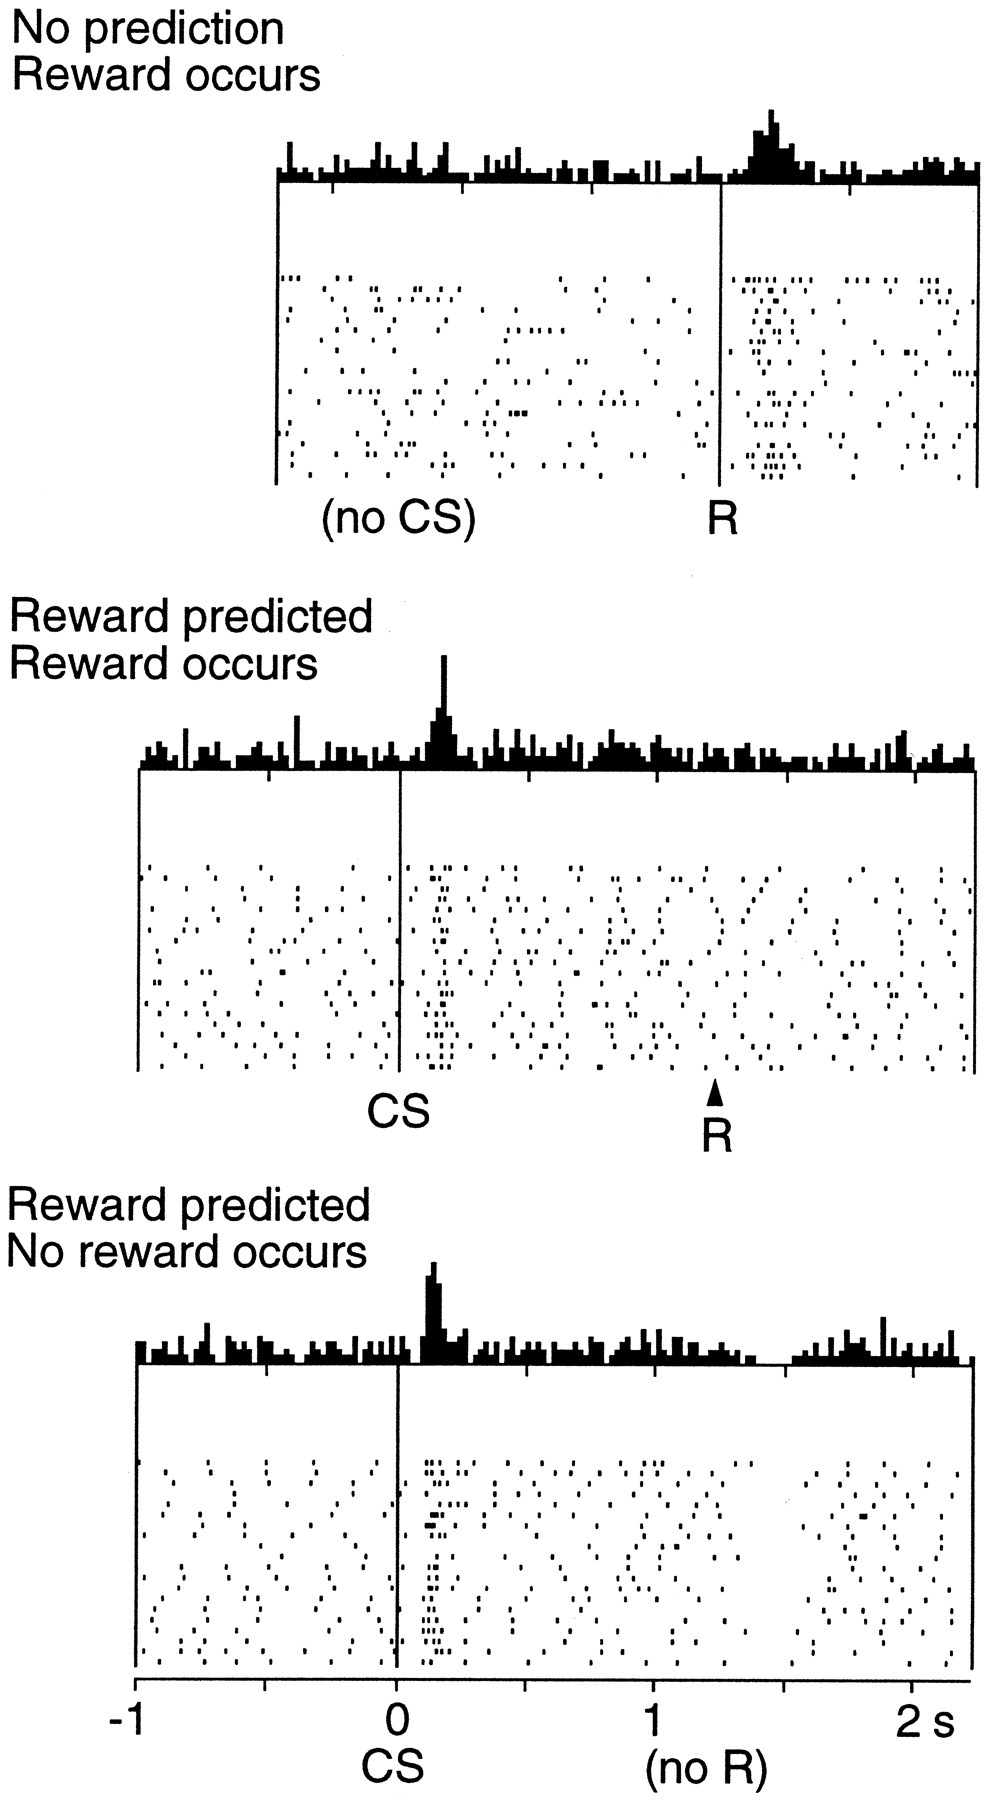
\includegraphics[width=0.60000\textwidth]{./figures/schultz.jpg}
\caption{Dopamine neurons implement a reward prediction error. When no
conditioned stimulus (CS) is presented, dopamine neurons fire in
response to a reward R (top panel). When a CS such as a light is
predictive of the reward, the dopamine response shifts to firing after
the CS instead (middle panel). If no reward is presented even though it
was predicted because of the light, there is a dip in the dopaminergic
neuron response at the time when the reward should have appeared. Figure
from Schultz et al. (1997), reprinted with permission from
AAAS.\label{fig_schultz}}
\end{figure}

While not uncontroversial (Redgrave, Gurney, \& Reynolds, 2008;
Redgrave, Prescott, \& Gurney, 1999), this finding of a direct neural
implementation of a prediction error and the close association between
dopamine and reinforcement learning has inspired a lot of research in
human neuroimaging, commonly attributing neural correlates of reward
prediction errors to the striatum (see e.g., Chase, Kumar, Eickhoff, \&
Dombrovski, 2015; Garrison, Erdeniz, \& Done, 2013 for recent reviews).

Several studies have shown that dopamine levels in the brain promote
associative learning in specific ways. Frank and colleagues, using a
probabilistic learning task, discovered that dopamine medication in
Parkinson's patients would make them better at learning from positive
than negative outcomes, while patients off medication showed the
opposite contrast (Frank, Seeberger, \& O'Reilly, 2004). Further,
polymorphisms in genes related to dopamine function also showed a direct
relation to positive and negative learning styles. For example,
participants with variations in dopamine D2 receptor densities displayed
differences in their proneness to learn from or generalize to negative
outcomes (Frank et al., 2007; T. A. Klein et al., 2007).

Computational modelling has been effectively used in combination with
neuroimaging methods like fMRI to elucidate e.g., developmental changes
in reinforcement learning (Van Den Bos, Cohen, Kahnt, \& Crone, 2012),
risk sensitivity (Niv, Edlund, Dayan, \& O'Doherty, 2012) and deviations
in reward learning in mental disorders like depression (Kumar et al.,
2008) and bulimia nervosa (G. K. W. Frank, Reynolds, Shott, \& O'Reilly,
2011). Neuroimaging studies provided additional evidence that striatum
and midbrain are involved in the computation of reward prediction errors
and implicate the ventromedial prefrontal cortex in the estimation of
values (Chase et al., 2015; Jocham, Klein, \& Ullsperger, 2011).

\section{The intersection of cognitive control and reinforcement
learning}\label{the-intersection-of-cognitive-control-and-reinforcement-learning}

How cognitive control processes can benefit value learning, override
action tendencies or sway neural processes to promote a more model-based
or model-free computation has only recently sparked investigations. For
example, in a recent study, cognitive control related measures in two
tasks were associated with a higher amount of model-based reward
learning in a two-stage reinforcement learning task (Otto, Skatova,
Madlon-Kay, \& Daw, 2015).

Yet, whether cognitive control can also have an impact on model-free
reinforcement learning is less well known. We have addressed this issue
in \textbf{Study I}, demonstrating that post-error slowing can have an
impact on the generalization of learning in a model-free reinforcement
learning paradigm (Schiffler, Almeida, Granqvist, \& Bengtsson, 2016).
Another study provided support that connectivity between anterior
cingulate cortex and ventromedial prefrontal cortex was associated with
adaptive switches in choice behaviour, integrating both immediate and
delayed consequences (Economides, Guitart-Masip, Kurth-Nelson, \& Dolan,
2014). This finding suggests a possible cognitive control process,
foregoing the immediate reward for a potentially larger delayed outcome.

Furthermore, the interaction between cognitive control and reward
learning plays an important role in mental disorders and can thus be a
potential future target for specific intervention. Particularly in
addiction, self-control over prepotent response habits is required to
sustain abstinence. Volkow and colleagues showed that instructed
cognitive control of drug craving activated right inferior frontal gyrus
as a node in a cognitive control network while inhibiting reward related
regions, including nucleus accumbens and orbitofrontal cortex (Volkow et
al., 2010). As compulsive disorders show a habit towards model-free at
the expense of model-based learning (Voon et al., 2015), further work on
the relation of cognitive control and reward learning styles could be
beneficial to illuminate the ways in which cognitive control can benefit
abstinence and ultimately recovery from these disorders.

\section{Challenges}\label{challenges}

\subsection{Is response adaptation like PES beneficial to
learning?}\label{is-response-adaptation-like-pes-beneficial-to-learning}

Whether PES provides specific benefits in acquisition or transfer in
learning paradigms is of yet unclear (Ullsperger \& Danielmeier, 2016;
Ullsperger et al., 2014). For example, it is still to be determined
under which conditions PES is associated with post-error accuracy
(Danielmeier \& Ullsperger, 2011; Hajcak, McDonald, \& Simons, 2003;
Hester, Barre, Mattingley, Foxe, \& Garavan, 2007).

We address these questions in our \textbf{Studies I} and \textbf{III}
(Schiffler et al., 2016; Schiffler, Bengtsson, \& Lundqvist, 2017),
investigating learning benefits of PES and how post-error decision
components relate to stabilisation of accuracy.

\subsection{How long do PES effects persist after an
error?}\label{how-long-do-pes-effects-persist-after-an-error}

A related question concerns for how long an error affects decision
making. In \textbf{Study I}, we investigated whether there was a memory
component to PES in a reinforcement learning task, i.e., whether
participants would adapt their response speed in relation to the
negative feedback on certain symbol pairs. In \textbf{Study II}, we
teased apart the effects of negative feedback on immediate next trials
and delayed adaptation on later trials with regards to anatomical
correlates. Finally, in \textbf{Study III} we investigated the
persistence of post-error adaptations several trials after the error in
a visual search task.

\subsection{What are the time courses and contributions to accuracy of
decision processes involved in
PES?}\label{what-are-the-time-courses-and-contributions-to-accuracy-of-decision-processes-involved-in-pes}

Previous studies have found to varying degree that both increases in
decision threshold and reduced sensitivity to sensory information
underlie PES. In \textbf{Study III}, we explored how these altered
decision components change over time and how they contribute to the
stabilisation of accuracy.

\section{Computational modelling to tackle these
challenges}\label{computational-modelling-to-tackle-these-challenges}

Advances in computer science, neuroscience and artificial intelligence
prompted a cognitive revolution in the 1950s which enabled psychology to
look beyond the black box of mental phenomena previously favoured by the
predominant field of behaviourism. One way to validate theories about
mental processes is to utilize computational models which can be fit to
behavioural and/or neural data acquired in experiments.

In this section I will present a general overview over the two main
models used in our studies. These are reinforcement learning models,
which try to explain how participants learn by estimating the stored
value of task items and predicting decisions based on these values and
drift diffusion models, which are fit to reaction times and accuracy in
a given task to illuminate the underlying decision process.

\subsection{Reinforcement learning
modelling}\label{reinforcement-learning-modelling}

The central theme in reinforcement learning modelling questions how the
value of rewards in the environment impacts decision making. The
Rescorla-Wagner model of animal learning formalized how the value of a
conditioned stimulus (CS) changes in a classical conditioning paradigm
dependent on the worth of the actual unconditioned stimulus (US)
(formula modified from Niv, 2009; Rescorla \& Wagner, 1972):

\[V_{new}(CS_i) = V_{old}(CS_i) + \alpha\left[\lambda_{US} - \sum_iV_{old}(CS_i)\right]\]

Here, learning of the association between US and CS happens because the
new value \(V_{new}(CS_1)\) of any of the conditioned stimuli (e.g., a
light as \(CS_1\)) gets updated by adding the difference between what
actually happened (e.g., a food pellet as \(\lambda_{US}\)) and what was
predicted - \(\sum_iV_{old}(CS_i)\) - to its old value
\(V_{old}(CS_1)\).

The importance of the difference between expected and predicted value
was a remarkable insight at the time and is one of the key components of
reinforcement learning models and other computational models of brain
function even today. It indicates the surprise of a particular outcome
and is additionally modulated by a learning rate \(\alpha\) which
reflects the importance of recency of rewards and can for example vary
depending on the salience of the stimuli involved (Niv, 2009).

This measure of surprise also found its way into reinforcement learning
models which are in active use in research today. In cognitive
neuroscience, the measure of the prediction error has received
particular attention because of its close relation with dopamine neuron
firing (Schultz et al., 1997) as well as its correspondence to
dissociable model-free (i.e., reward-related) and model-based (i.e.,
state-related) correlates in the brain (Gläscher et al., 2010).
Analogous to the final term in the Rescorla-Wagner model, the prediction
error can be calculated as follows by subtracting the expected value of
a stimulus \(V\) at timestep \(t\) from the current value \(r\) at
timestep \(t\):

\[\delta_t = r_t - V_t\]

The full equation with which value updates can be estimated then looks
like this:

\[V_{t+1} = V_t + \alpha * \delta_t\]

How do these stimulus values lead to a decision towards one or another
option? The computed values can be converted to action probabilities by
the softmax equation, in which for example the probability of choosing
between stimulus A and B at time \emph{t} can be described as follows:

\[P(A)_t = \frac{1}{1 + e^{-\beta(V(A)_t - V(B)_t)}}\]

In this formula, the difference between the values of stimuli A
(\(V(A)_t\)) and B (\(V(B)_t\)) is computed and adjusted by the inverse
temperature parameter \(\beta\), which controls individuals' propensity
to explore new options versus exploit the known value differences
(albeit small as they might be). In other words, an increase in the
value for \(\beta\) suggests that a participant follows the computed
value difference more deterministically.

RL models have already been effectively applied to highlight previously
unexplained aspects of disorders (for a review see Maia \& Frank, 2011)
such as Parkinson's disease (Frank et al., 2004), Schizophrenia (Roiser
et al., 2009) and in explaining model-based versus model-free behaviour
(Doll, Simon, \& Daw, 2012) which might be of future use to explain
pathologies.

\subsection{Drift diffusion modelling}\label{drift-diffusion-modelling}

The fundamental question how mental computations can be inferred from
measured reaction times dates back almost 150 years. Already in 1870 and
based on earlier computations on nerve conduction velocity by von
Helmholtz (1850), Foster described the principle on which today's drift
diffusion models (DDM) base their computations, namely the division of
overt reaction time into the unobservable components of sensory
acquisition, mental computation, and motor output: ``A typical bodily
action, involving mental effort, may be regarded as made up of three
terms ; of sensations travelling towards the brain, of processes thereby
set up within the brain, and of resultant motor impulses travelling from
the brain towards the muscles which are about to be used'' (Foster,
1870).

Modern sequential sampling models, of which DDMs are one subclass, rely
on the idea that during speeded decision-making tasks, evidence towards
one of the options is acquired in a noisy manner until it reaches a
decision boundary, after which a motor action is being executed
(Forstmann, Ratcliff, \& Wagenmakers, 2016). DDMs have usually been
applied to two-alternative forced choice tasks (2AFC), although
extensions to include tasks with multiple alternatives have also been
discussed (Forstmann et al., 2016; Ratcliff, Smith, Brown, \& McKoon,
2016).

\begin{figure}
  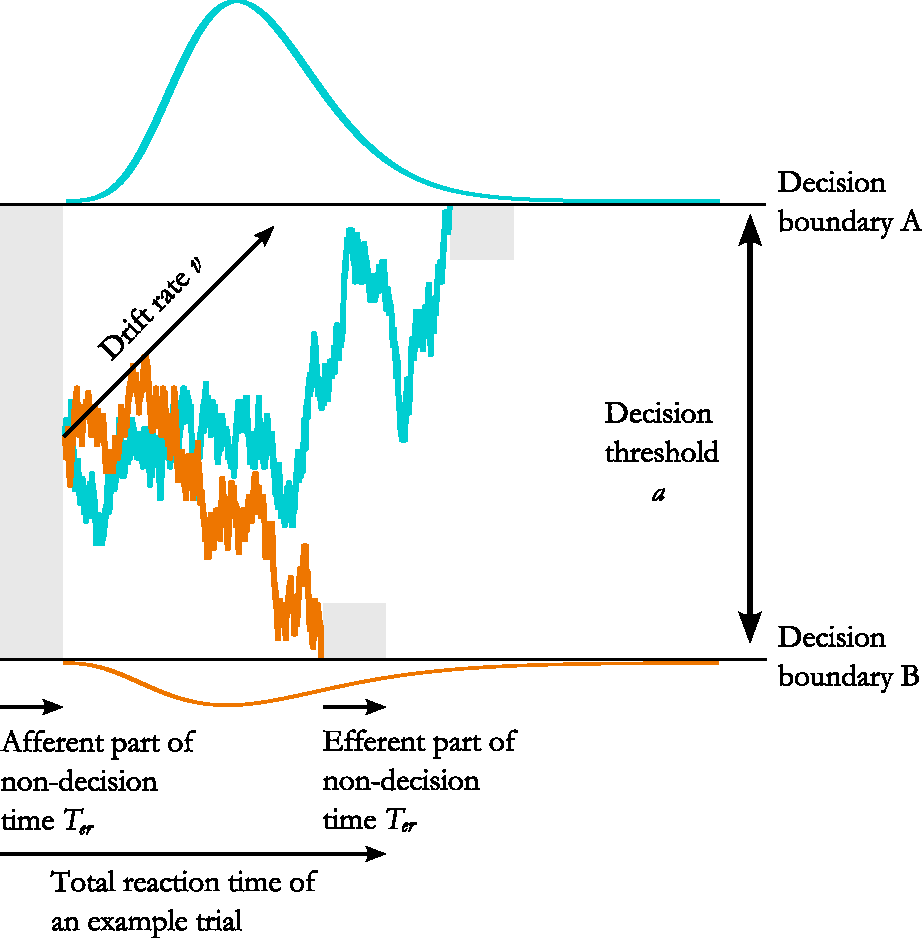
\includegraphics{./figures/ddm.pdf}
  \caption{Main parameters of the canonical drift diffusion model for decisions in two-alternative forced-choice tasks. Two example diffusion processes as random walks are depicted alongside the three main parameters of the drift diffusion model. Evidence for one or the other option is accumulated with a drift-rate $v$ until one of the two decision boundaries which are separated by the decision threshold $a$ is crossed. The total non-decision time $T_{er}$ can be divided in an afferent part (sensory perception) and an efferent part (movement initiation and execution).\label{fig_ddm}}
\end{figure}

Prominent parameters in these models include the decision threshold
\emph{a}, the rate of evidence accumulation \emph{v}, and the
non-decision time \emph{T\textsubscript{er}}, which consists of time
needed for both sensory acquisition as well as motor execution (see
Figure \ref{fig_ddm} for a graphical overview of the DDM and its core
parameters). While \emph{a} reflects how much evidence is necessary to
make a decision towards one of the options presented, \emph{v} indicates
the slope at which this evidence is acquired.

These three parameters relate to RT and accuracy in a particular fashion
(Table \ref{tbl1}). The decision threshold \emph{a} corresponds to
increases in response caution with an increase in both RT and accuracy.
The evidence accumulation \emph{v} is related to decreases in RT and
simultaneous increases in accuracy and is sensitive to for example task
difficulty (higher difficulty leads to decreased \emph{v}). Finally, the
non-decision time \emph{T\textsubscript{er}} corresponds to an increase
in RT with no concurrent change in accuracy and is hypothesized to be
for example affected by aging (Ratcliff, Thapar, \& McKoon, 2010),
although Ratcliff et al. (2010) also find increasing decision thresholds
with advancing age.

\begin{longtable}[]{@{}lccc@{}}
\caption{Core parameters of drift diffusion models and their relation to
RT, accuracy, and proposed correlates.\label{tbl1}}\tabularnewline
\toprule
DDM Parameter & RT & Accuracy & Proposed correlates\tabularnewline
\midrule
\endfirsthead
\toprule
DDM Parameter & RT & Accuracy & Proposed correlates\tabularnewline
\midrule
\endhead
Decision threshold \emph{a} & ↑ & ↑ & Response caution\tabularnewline
Drift rate \emph{v} & ↓ & ↑ & Task difficulty\tabularnewline
Non-decision time \emph{T\textsubscript{er}} & ↑ & = &
Aging\tabularnewline
\bottomrule
\end{longtable}

Using reaction time distributions and response accuracy in combination
allows for example to explain differences in experimental conditions
(Forstmann et al., 2016 for reviews; see Ratcliff et al., 2016) or
between patient groups, such as in schizophrenia (A. A. Moustafa et al.,
2015), Parkinson's disease (Zhang et al., 2016) or in patients with
psychosis (Mathias et al., 2017) to particular mental processes within
the total reaction time.

\chapter{Aims}\label{aims}

The central aim of the studies presented in this thesis was to
investigate which aspects of cognitive control processes in reaction to
negative feedback benefit learning and how this is reflected in both
brain anatomy and function.

In \textbf{Study I} we used a probabilistic reinforcement learning
paradigm to assess the influence of cognitive control adjustments such
as post-error slowing and stay/switch-behaviour in addition to learning
phase performance as predictors for learning outcome in a later test
phase. In addition, we were interested in which neural areas predicted
later response time adaptation at the time of receiving negative
feedback. Further, we analyzed how trial-by-trial absolute and signed
prediction errors obtained from our reinforcement learning models
affected behaviour and how they were represented in the brain. Data for
this study was acquired in the context of a larger ongoing project which
investigates the influence of self-associations on learning using
priming techniques. Therefore we controlled for this factor in all
analyses of \textbf{Studies I} and \textbf{II} in which this was
possible.

Given converging evidence from previous research (e.g., Aron et al.,
2007, 2014; Rae et al., 2015) and the interesting results from
\textbf{Study I} which implicated the right inferior frontal cortex as
an important region in cognitive control processes, we investigated in
\textbf{Study II} whether an anatomical property of this area, cortical
thickness, was related to the extent and memory aspects of PES. We also
used drift diffusion modelling to better understand the dominant
cognitive process behind post-error slowing and related obtained
parameters to anatomical structure of the rIFC.

Using a visual search task, in \textbf{Study III} we explored the effect
of an error on not only the first trial after the error, but also on
subsequent trials. This was again supported by drift diffusion models to
reveal the relevant decision process components behind reaction times
and accuracy. Additionally, we examined how trial type properties
(emotion and difficulty) influenced post-error adaptations and how later
increases in accuracy were associated with decision processes on the
trial after an error.

\chapter{Methodological
Considerations}\label{methodological-considerations}

In this chapter I will provide an outline of the main techniques used in
our studies with a focus on neuroimaging techniques and computational
modelling.

\section{Magnetic Resonance Imaging}\label{magnetic-resonance-imaging}

Magnetic Resonance Imaging (MRI) is a non-invasive imaging technique
that utilizes the fact that different tissue types have different
magnetic properties to provide high-resolution images of anatomy such as
the brain. To make this possible, a strong magnetic field, commonly in
the range of 1.5 - 7 Tesla for human brain imaging, is created by an MRI
scanner, which aligns the nuclei of (e.g., hydrogen) atoms in a common
direction. The transient introduction of a varying electromagnetic field
(B\textsubscript{1}) by a radiofrequency pulse leads to excitation and a
dephasing of the nuclei. Now it becomes for example possible to measure
how long it takes the nuclei to return back to their original state (the
so-called \emph{spin-lattice relaxation time} or
\emph{T\textsubscript{1}} relaxation). This property is used in
neuroimaging to provide the so-called \emph{T\textsubscript{1}}
contrast, which enables a detailed visualization of differences between
e.g., grey and white matter in the brain. We make use of the
\emph{T\textsubscript{1}} contrast in \textbf{Study II} to assess
inter-subject differences in cortical thickness depending on individual
propensity to adapt response speed after an error.

\begin{figure}
\centering
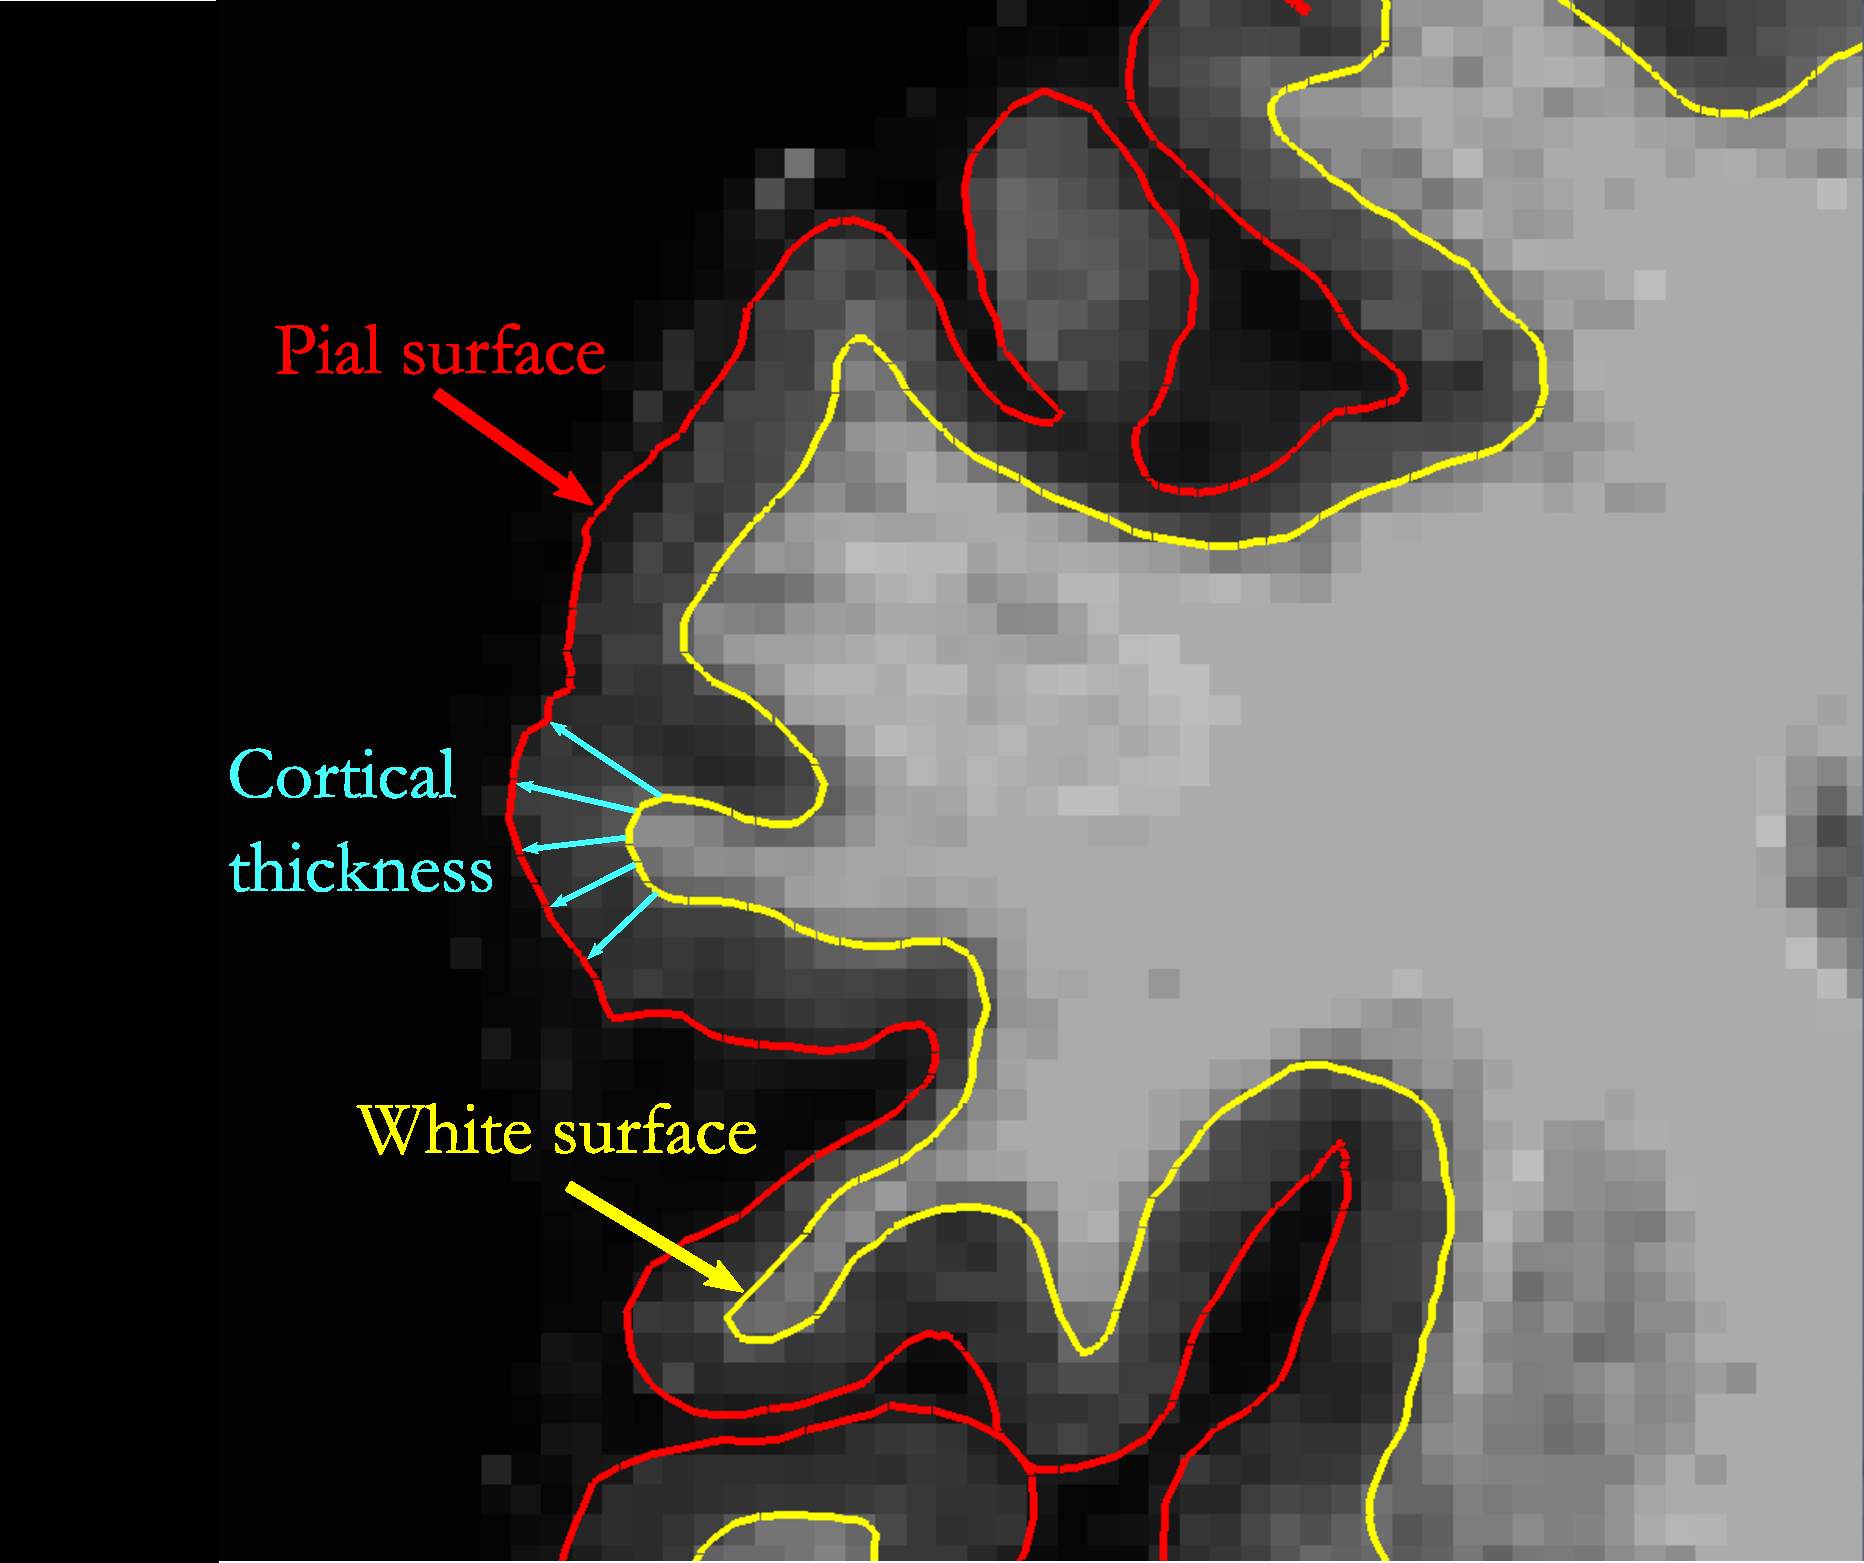
\includegraphics{./figures/cortical_thickness_freesurfer.pdf}
\caption{Cortical thickness is calculated using the shortest distance between pial surface and white surface. Image was created with the tool TkMedit after running the FreeSurfer standard processing pipeline on one example brain from Study II.\label{fig_corticalthickness}}
\end{figure}

Cortical thickness is a MRI-derived metric which has been successfully
used as a measure of the integrity of the cerebral cortex (e.g.,
Dickerson \& Wolk, 2012; Makris et al., 2007). It decreases with normal
aging (Storsve et al., 2014) and can be related to symptom severity with
corresponding regionally specific rates of decrease in Alzheimer's
disease (Dickerson et al., 2009). Using freely available tools such as
FreeSurfer (Fischl \& Dale, 2000), cortical thickness can be calculated
by taking the smallest distance between the pial surface (boundary
between grey matter and cerebrospinal fluid) and the white surface
(boundary between grey matter and white matter), as detailed in Figure
\ref{fig_corticalthickness}.

\section{Functional Magnetic Resonance
Imaging}\label{functional-magnetic-resonance-imaging}

Ideally, in cognitive neuroscience we would like to observe neuronal
activity directly and relate it to ongoing cognitive processes as for
example probed in closely controlled experimental studies. However, this
is not yet possible in a non-invasive fashion today. Instead, we use a
proxy to neuronal activity, the so-called Blood Oxygen Level Dependent
(BOLD) contrast (Ogawa, Lee, Kay, \& Tank, 1990). This contrast relies
on the fact that the deoxyhemoglobin concentration in the blood changes
when more oxygen is being consumed, for example because the participant
is currently doing a decision-making task and active brain areas need to
be supplied with more oxygen. This physiological change in
deoxyhemoglobin concentration changes the magnetic properties of water
molecules which is then measurable by MRI. The concept of BOLD-based
functional MRI (fMRI) relies on this indirect measure to assess neural
activity in the form of local field potentials (Logothetis, Pauls,
Augath, Trinath, \& Oeltermann, 2001). We make use of fMRI and the BOLD
contrast in particular in \textbf{Study I} using Statistical Parametric
Mapping (SPM, Wellcome Trust Centre for Neuroimaging, UCL, London,
United Kingdom) as the analysis tool.

\section{Reinforcement Learning
Modelling}\label{reinforcement-learning-modelling-1}

We used a standard RL model in \textbf{Study I} to investigate
participant's choices and their learning progress. Because we assumed
that participants learn differently from positive and negative feedback,
we estimated two learning rates, \(\alpha_{pos}\) and \(\alpha_{neg}\),
respectively. We initialized all weights at 0, the two learning rates at
0.5 (with \(0 \leq \alpha \leq 1\) and a beta distributed prior) and the
inverse temperature parameter \(\beta\) at 1 (with \(\beta \geq 0\) and
a normal distributed prior with mean = 0 and standard deviation =
\(\sqrt{10}\)).

On a trial-by-trial basis, stimulus values were estimated via the
following formula:

\[Q_{t+1} = Q_t + \alpha_{(pos/neg)} * \delta_t\] with the prediction
errors \(\delta_t\) calculated as:

\[\delta_t = r_t - Q_t\] Action probabilities (here for symbol A in pair
AB) were estimated using the softmax equation:

\[P(A)_t = \frac{1}{1 + e^{-\beta(Q(A)_t - Q(B)_t)}}\]

Further, we calculated a trial-by-trial confidence measure by putting
the action tendency estimated in the softmax equation in relation to
0.5:

\[Conf(AB)_t = | 0.5 - P(A)_t |\]

\section{Hierarchical Bayesian Estimation of the Drift Diffusion Model
(HDDM)}\label{hierarchical-bayesian-estimation-of-the-drift-diffusion-model-hddm}

To model latent decision processes of PES in \textbf{Studies I} and
\textbf{II} we used a toolbox which allows the estimation of the drift
diffusion model in a hierarchical Bayesian fashion (HDDM, Wiecki, Sofer,
\& Frank, 2013). In contrast to traditional ways of estimating diffusion
models, the hierarchical Bayesian analysis assumes that parameters for
individuals can be drawn from the group distribution and that an
uncertainty around the parameters can also be estimated. A major benefit
of this type of analysis is that far fewer trials per condition are
needed for each individual participant to get reasonable parameter
estimates as the individual parameter estimates are constrained by the
group estimates (Ratcliff \& Childers, 2015; Wiecki et al., 2013). In
our studies, we mainly focused on the three main parameters of the DDM:
The decision threshold \emph{a}, the rate of evidence accumulation
\emph{v}, and the non-decision time \emph{T\textsubscript{er}}. The
reaction time slowing after an error can be described by either an
increase in decision threshold, a decrease in evidence accumulation or
an increase in the non-decision time, see Figure
\ref{fig_ddm_pes_changes}. Teasing these contributions apart was
particularly our goal in \textbf{Study III}.

\begin{figure}
\centering
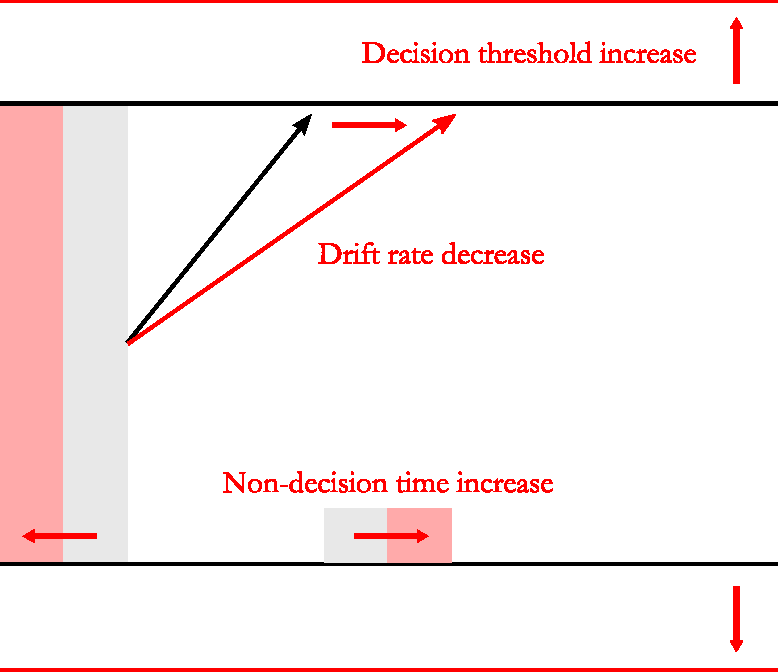
\includegraphics[height=0.80000\textwidth]{./figures/ddm_PES_changes.pdf}
\caption{Purported decision process changes underlying post-error
slowing. All three changes portrayed lead to a decrease in RT. However,
changes in the respective parameters of the drift diffusion model map
uniquely to changes in accuracy. While decision threshold increases
predict corresponding increases in accuracy, decreases in evidence
accumulation will lead to lower accuracy, and changes in non-decision
time do not affect accuracy.\label{fig_ddm_pes_changes}}
\end{figure}

\section{Post-error slowing}\label{post-error-slowing}

Traditionally, post-error slowing has been calculated by comparing
average RT on post-error trials with average RT on post-correct trials.
However, this method neglects the fact that errors might also cluster in
certain parts of the experiment, e.g., at the end when general attention
is low because participants are getting tired. It is therefore advisable
to take this into account and subtract post-error RTs from associated
pre-error RTs (so-called \(\Delta\)RT) instead so that global
fluctuations over the course of the experiment are being taken into
account (Dutilh et al., 2012a). In our studies, we also control for
trial type differences in RT by comparing trials of the same trial
condition. For \textbf{Studies I} and \textbf{II}, we calculate PES in
accordance with previous research on post-error slowing in a
reinforcement learning task design (Cavanagh et al., 2010; Frank et al.,
2007) by subtracting post-error RT for the next same pair from RT on the
error trial. For \textbf{Study III}, we calculate PES by subtracting
post-error RT from pre-error RT if they are of the same trial type
(neutral/angry/happy).

\section{Participants}\label{participants}

For \textbf{Studies I} and \textbf{II} we recruited a total of 48
healthy participants who gave written informed consent before
participating in the study. In \textbf{Study III}, 6,047 participants
took part in the study which was presented at an art exhibition at
Nationalmuseum in Stockholm, Sweden. Detailed information about the aims
of the research was given to participants both on the TV screen for the
experiment and on text panels of the installation and consent was
implied by participants voluntarily initiating the task.

\chapter{Results}\label{results}

\section{Study I: Post-error slowing is associated with learning
performance and functional activity in cognitive control and visual
regions}\label{study-i-post-error-slowing-is-associated-with-learning-performance-and-functional-activity-in-cognitive-control-and-visual-regions}

\subsection{Relation of learning phase measures to the testing
phase}\label{relation-of-learning-phase-measures-to-the-testing-phase}

In a multiple regression model, we found that both learning phase
accuracy on the main symbol pair (AB) and PES during the learning phase
were positively associated with testing phase performance (Correlation
between PES during learning phase and test score in Figure
\ref{fig_results_study1}A), while the number of times participants
decided to stay with the same decision after negative feedback or switch
to the other option was not directly related to test phase performance.

\begin{figure}
  \centering
  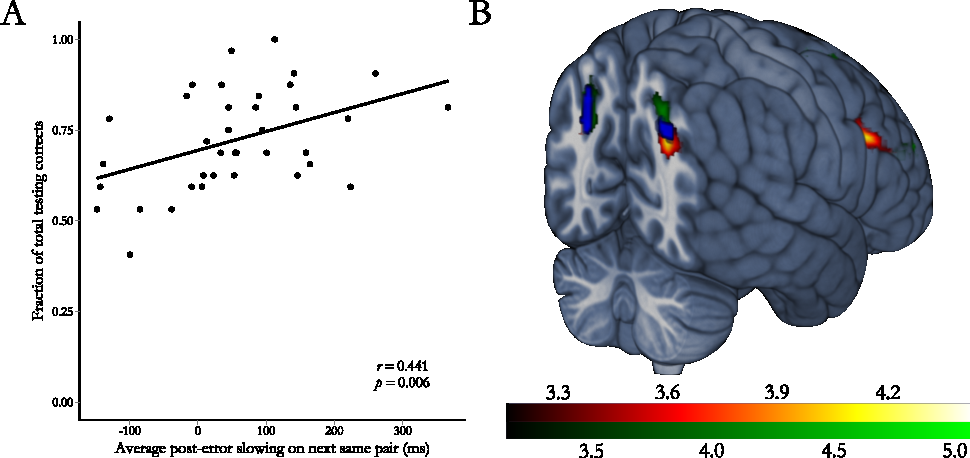
\includegraphics{./figures/results_study1.pdf}
  \caption{Main results of Study I. (A) Positive correlation between memory-based post-error slowing and test phase performance across participants. (B) fMRI activity of brain areas while receiving negative feedback, related to amount of slowing on the next same pair trial (red-yellow) and to absolute prediction error (green), as well as the conjunction between both (blue). Figures from Schiffler et al., 2016, reprinted with permission from MIT Press.\label{fig_results_study1}}
\end{figure}

We did not find a correlation of PES with overall accuracy of any of the
symbol pairs during the learning phase. Testing phase scores also
demonstrated that participants performed better in the test phase on new
symbol combinations which were easier. For example, the choice between
symbol A which was reinforced at an 80\% probability during the learning
phase and symbol D, which was reinforced at 30\% should be easier than
the choice between A and C (80\%/70\%), see Figure \ref{fig_testscores}.

\begin{figure}
  \centering
  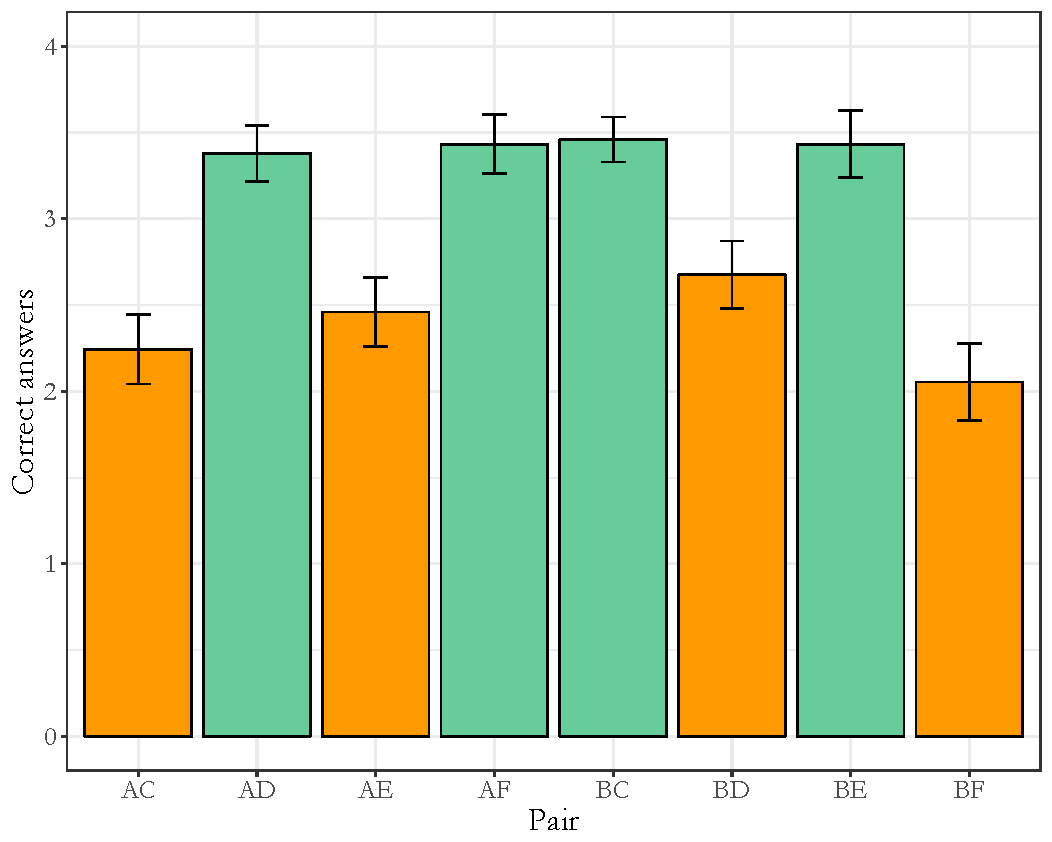
\includegraphics[height=0.70000\textwidth]{./figures/test_scores_by_pair_se.pdf}
  \caption{Test scores divided by symbol pair combinations. During the test phase of the task, the symbols A and B from the learning phase are now tested separately against all other symbols learned. Green colour represents easier symbol combinations (AD: 80\%/30\% probability of positive reinforcement, AF: 80\%/40\%, BC: 20\%/70\%, BE: 20\%/60\%) and orange represents more difficult combinations (AC: 80\%/70\%, AE: 80\%/60\%, BD: 20\%/30\%, BF: 20\%/40\%). Error bars reflect standard error of the mean.\label{fig_testscores}}
\end{figure}

\subsection{Feedback-congruent
staying/shifting}\label{feedback-congruent-stayingshifting}

As expected, participants on average repeated decisions more often when
they were reinforced by positive feedback compared to negative feedback.
A general working memory component as indicated by feedback congruent
behaviour in the beginning of the task (Frank et al., 2007) was not
significantly related to PES.

\subsection{fMRI activity associated with
PES}\label{fmri-activity-associated-with-pes}

On the event of receiving negative feedback, activity in right inferior
frontal cortex and bilateral occipital cortex tracked the response speed
adjustment on the following relevant trial (Figure
\ref{fig_results_study1}B).

\subsection{Reinforcement learning model
measures}\label{reinforcement-learning-model-measures}

\subsubsection{Prediction errors and their neural
correlates}\label{prediction-errors-and-their-neural-correlates}

Prediction errors estimated from our reinforcement learning model were
associated with post-error slowing. More unexpected negative feedback
lead to an increase in slowing both on the direct next trial and on the
next relevant (same pair) trial while more unexpected positive feedback
was followed by a speed increase. Negative prediction errors correlated
with brain activity in left striatum as assessed by an \emph{a priori}
ROI analysis and absolute (i.e., unsigned) prediction errors over all
feedback evoked activity in similar brain regions as the main PES
analysis.

\subsubsection{Learning rate}\label{learning-rate}

We had estimated two separate learning rates for positive and negative
feedback in accordance with previous research (Kahnt et al., 2009; Van
Den Bos et al., 2012) to investigate whether participants who showed
stronger reactivity to negative feedback (e.g., increased slowing or
switching to the other symbol) showed a learning pattern which focuses
on recent feedback in contrast to the whole history (i.e., a high
learning rate). We found this pattern for switch behaviour, but not for
post-error slowing. This means that the model estimated a higher
negative learning rate for participants who switched their choice to the
other symbol following negative feedback.

\subsubsection{Confidence}\label{confidence}

Confidence measures as extracted by our RL model also showed a negative
relation to PES (i.e., lower confidence lead to an increase in
\(\Delta\)RT).

\subsubsection{Model validation}\label{model-validation}

We simulated model predictions by taking the final model parameters
(\(\alpha_{pos,neg}\) and \(\beta\)) and averaged over 10,000
repetitions of simulated behaviour for each participant. The model was
able to reproduce the learning curves present in the acquired data as
well as the differentiation in accuracy between the three different
symbol pairs at the end of the training phase.

\section{Study II: Adaptive increases in response caution after errors
are related to cortical thickness in cognitive control
regions}\label{study-ii-adaptive-increases-in-response-caution-after-errors-are-related-to-cortical-thickness-in-cognitive-control-regions}

\subsection{Drift diffusion correlates of PES in a reinforcement
learning
design}\label{drift-diffusion-correlates-of-pes-in-a-reinforcement-learning-design}

Post-error trials, compared to post-correct trials, were defined by an
increase in decision threshold but there was no difference in the rate
of evidence accumulation (Figure \ref{fig_results_study2}A,B).

\begin{figure}
\centering
  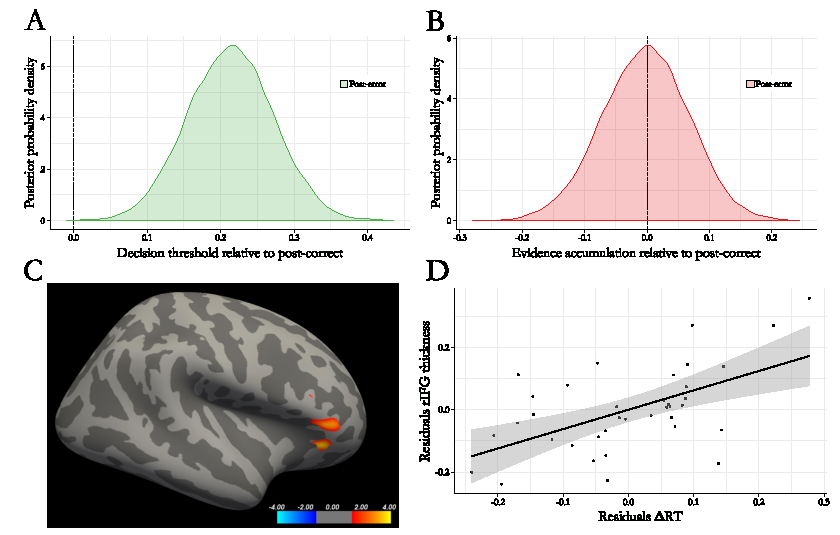
\includegraphics{./figures/results_study2.pdf}
  \caption{Main results of Study II. (A) Posterior probability density of decision threshold parameter regression estimate for post-error trials compared to post-correct trials. (B) Posterior probability density of evidence accumulation parameter regression estimate for post-error trials compared to post-correct trials. (C) Vertex based analysis showing clusters in which rIFG thickness is positively associated with $\Delta$RT. (D) Correlation between average $\Delta$RT and average rIFG cortical thickness when partialing out the effects of age, sex and prime. Shaded area indicates 95\% confidence interval of the regression line.\label{fig_results_study2}}
\end{figure}

This indicates that error trials evoke increased response caution in
this task design but not necessarily decreases in evidence accumulation.
Against our expectations, an interaction between the distance to the
next same pair trial and the rate of evidence accumulation was not
supported by the data. These findings suggest that memory-based PES is
an adaptive cognitive control process because the RT increases in this
experiment contributed to accuracy as shown by the increase in response
caution.

\subsection{PES is related to cortical thickness in
rIFC}\label{pes-is-related-to-cortical-thickness-in-rifc}

We found that overall cortical thickness of rIFC correlated with PES,
both if the same pair was the direct next trial after the error and if
there was at least one other symbol pair in between. \emph{Post-hoc}
correlations and a follow-up vertex wise analysis both demonstrated that
the strongest association of PES was to the anterior part of rIFC
(Figure \ref{fig_results_study2}C,D), in pars orbitalis (particularly
for longer distances) and pars triangularis (especially for immediate
next trials).

\subsection{Response caution increases after errors directly relate to
cortical thickness in
rIFC}\label{response-caution-increases-after-errors-directly-relate-to-cortical-thickness-in-rifc}

Using participants' parameters of decision threshold and evidence
accumulation adaptation on post-error trials compared to post-correct
trials, we showed that anatomical variability in rIFC, particularly in
pars orbitalis, related to decision threshold adaptations on the trial
after the error.

\section{Study III: Response adaptations to errors are multi-component
processes and change dynamically over several trials after the
error}\label{study-iii-response-adaptations-to-errors-are-multi-component-processes-and-change-dynamically-over-several-trials-after-the-error}

\subsection{Dynamics of latent decision processes after
errors}\label{dynamics-of-latent-decision-processes-after-errors}

In this study, we have found that reactions are marked by sustained
increases in response caution over several trials and transient
decreases in evidence accumulation, most prominent on the direct next
trial after the error (Figure \ref{fig_results_study3}A).

\begin{figure}
  \centering
  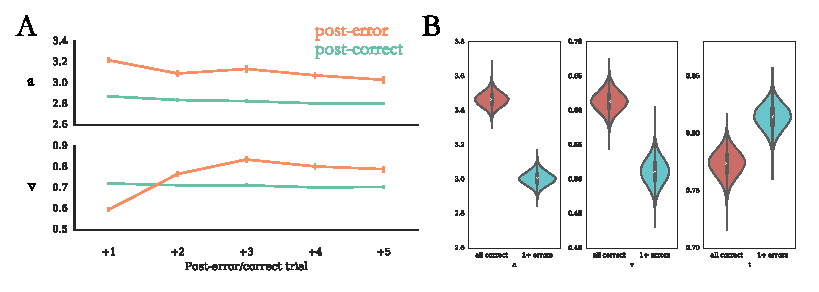
\includegraphics{./figures/results_study3.pdf}
  \caption{Main results of Study III. (A) Decision process components contributing to post-error slowing over several trials after an error. While decision threshold $a$ showed a sustained increase even several trials after an error (orange) compared to post-correct trials (green), an initial post-error dip in evidence accumulation $v$ increased over the following trials. Non-decision time $T_{er}$ (not shown) displayed a sustained decrease for post-error trials relative to post-correct trials. (B) Relation of decision process parameters on the first trial after an error to accuracy on the following five trials. Higher decision thresholds $a$ and evidence accumulation $v$ as well as lower non-decision time $T_{er}$ immediately post-error were associated with no mistakes on the following five trials compared to at least one mistake. Figures from Schiffler et al., 2017, adapted under CC BY 4.0 license.\label{fig_results_study3}}
\end{figure}

Further, we also found that non-decision time was reduced for several
trials post-error. This indicates that in our experiment, multiple
decision processes were affected simultaneously by the error and give
rise to the particular pattern of post-error slowing.

\subsection{How do downstream accuracy increases rely on post-error
adaptation?}\label{how-do-downstream-accuracy-increases-rely-on-post-error-adaptation}

Post-error trials which were followed by five correct trials were marked
by higher decision thresholds, higher rates of evidence accumulation and
lower non-decision times (Figure \ref{fig_results_study3}B).

\subsection{Effects of error properties on decision
making}\label{effects-of-error-properties-on-decision-making}

We found differences in post-error decision processes both by emotional
valence and difficulty of stimuli. These variations had specific effects
on the rate of evidence accumulation. It was reduced both for generally
more difficult trials and following angry error trials compared to happy
error trials.

\chapter{Discussion}\label{discussion}

Can appropriate response adaptation to negative feedback support
learning? Our studies presented in this thesis suggest that this is
indeed generally the case, but that there are also potentially
detrimental components which need to be recognized.

\section{Behavioural results in Studies I -
III}\label{behavioural-results-in-studies-i---iii}

In \textbf{Studies I} and \textbf{II} we have presented evidence that
PES in a RL context can benefit learning outcome. \textbf{Study I}
demonstrated that there are long-term learning outcome benefits if
participants adapt their response speed to the negative feedback
received. Interestingly, the effect that we found for PES on testing
phase performance was similar in magnitude to the effect of overall
learning phase performance in the main symbol pair AB on the test score.
This is somewhat surprising as being able to clearly differentiate
between the value of these two symbols as indicated by accuracy on pair
AB during the learning phase should be a strong predictor for
performance during the test phase in which symbols A and B are
separately pitted against all other symbols.

These findings extend the literature on beneficial and adverse effects
of PES on learning by showing that error monitoring processes after
negative feedback can be an indicator for later learning outcome as
stipulated by Ridderinkhof and colleagues (2004). This suggests that
negative feedback is encoded at the time of receiving the feedback to
drive future response adaptations. This finding emphasizes encoding of
feedback as a crucial phase for subsequent changes in behaviour, which
may have implications for structuring learning exercises, e.g., in the
classroom.

In \textbf{Study II}, we showed that PES also has a positive effect
during the initial learning phase of the task. The increase in RT was
associated with an increase in the decision threshold, which signals
that participants made more cautious (and thus on average more correct)
decisions after errors. This finding is not very surprising, given that
post-error adaptations in general have previously been associated with
increases in response caution (Dutilh et al., 2012b) and that in a
different reinforcement learning task, decision threshold has been
linked to decision conflict (Frank et al., 2015). The result reiterates
that the additional time that is often being taken after errors is
beneficial to learning performance.

\textbf{Study III} provided evidence for both functional and potentially
maladaptive decision components in the process of post-error slowing.
While response caution persisted at elevated levels even several trials
after the error, reductions in evidence accumulation were mainly present
for the first post-error trial, suggesting only a transient disruption
of decision making by the error.

Reduced evidence accumulation and increased decision boundaries have
also been found in a motion direction discrimination task (Purcell \&
Kiani, 2016), although that study did not find any differences in
non-decision time. However, in our case, the non-decision time was
reduced following errors, i.e., this part of the decision process did
not contribute to post-error slowing.

Our findings align with a recent conceptual proposal, which suggests
both co-occurring increases in response threshold and decreases in
sensitivity to sensory information which together lead to initial
decreases in accuracy and eventual recovery over future trials
(Ullsperger \& Danielmeier, 2016).

Interestingly, these results as predicted by the aforementioned theory
stand in contrast to Laming's (1979) original findings that RT recovers
faster after an error than task accuracy, possibly due to differences in
the task being used or in the way that post-error slowing was
calculated.

\section{Neuroimaging results in Studies I and
II}\label{neuroimaging-results-in-studies-i-and-ii}

In \textbf{Studies I} and \textbf{II}, we show that PES was associated
with both function and anatomy of the rIFG, an important cognitive
control region in the brain. Specifically, anatomical variability in
cortical thickness in this area reflected participants' decision
threshold adaptations after errors, suggesting a possibility that there
are markers of propensity to error adaptation in the human brain which
can be investigated in further research. Functional activity in rIFG
when receiving the error feedback was positively associated with
response time slowing on the next relevant trial.

In similar previous analyses, activity in dorsolateral PFC (Kerns et
al., 2004) and pMFC (Danielmeier et al., 2011) on the error trial
predicted RT slowing on the post-error trial. Hester and colleagues also
demonstrated that error activity in pMFC predicted accuracy on the next
same target stimulus, even if that trial was several trials ahead in the
future (Hester, Madeley, Murphy, \& Mattingley, 2009). Further, activity
in bilateral IFG has previously been associated with successful
instrumental learning (Guitart-Masip et al., 2012).

It is unlikely that there exists only one single region in PFC which
determines response adaptations like PES, but that instead several areas
cooperate to implement the response speed adjustments in cooperation
with primary motor areas, the pre-SMA and subcortical regions like the
STN (Siegert et al., 2014). Further, these areas likely interact with
regions which have been consistently shown to be involved in error
monitoring like pMFC and ACC. Our contribution in the studies presented
here is that lateral PFC, and more specifically rIFG, is directly
involved in signalling the need for a future more cautious response
after receiving the feedback, not only for suppressing the motor output
on the post-error trial. Future studies which focus on functional or
anatomical network approaches (as e.g., in Rae et al., 2015) will be
able to provide a more comprehensive answer to these questions.

\section{Limitations and future
directions}\label{limitations-and-future-directions}

Particularly for our drift diffusion modelling we have employed a method
which enables accurate parameter estimation even when trial amounts are
low. However, for the particular conditions we wanted to investigate, we
still encountered problems in convergence and had to make compromises on
the model structure (i.e., model the data on group level in
\textbf{Study III} and reduce model complexity in \textbf{Study II}) to
assure convergence of the models. Even though we had a lot of
participants in \textbf{Study III} and the direction of almost all
parameter estimates when including individual level modelling was the
same as for the group models, the trial amount per participant should
still be increased to also get stable individual parameter estimates.

Further, it is important to consider that the PES effects we have
observed here differ between the presented studies due to the
intricacies of the two experimental designs. Particularly, this concerns
the memory-based aspect of PES in \textbf{Study I} and \textbf{II}
compared to a more conventional visual search task in \textbf{Study
III}. While adaptation of response speed in line with previous relevant
feedback is reasonable and has previously been found in other studies
employing the same type of probabilistic reinforcement learning task
(Cavanagh et al., 2010; Frank et al., 2007), this might constitute a
different aspect of PES than what has historically been classified as
PES. For example, one recurring finding in PES research (Danielmeier \&
Ullsperger, 2011; see e.g., Jentzsch \& Dudschig, 2009) is that the
slowing is greater when the response to stimulus interval is smaller
(i.e., the closer the time from feedback to onset of next stimulus). In
our first two studies, a considerable amount of time could pass between
a particular feedback and the next relevant trial (on average 20 seconds
between feedback and next same pair in comparison to traditional studies
of PES in which the response to stimulus interval is usually below one
second). As such, the received negative feedback needs to be stored in
some way until the participant recognizes the same pair for the next
time. What we investigate in the first two studies could thus involve a
more cognitive aspect of post-error slowing than has been conventionally
examined.

In \textbf{Study I} and \textbf{II}, the PES effect was also
comparatively smaller to PES in \textbf{Study III}. This might be
because there were few error trials in the latter study which bias the
analysis of post-error reactions towards initial encounters of errors.
Conceivably, these initial errors might provoke a stronger post-error
reaction, but this hypothesis would need to be tested in future studies.

Another interesting aspect for future research concerns the question how
errors in deterministic decision-making tasks differ from probabilistic
negative feedback often given in reinforcement learning task designs
with regard to involvement of brain areas associated with cognitive
control. One possibility is that while the former feedback evokes a
similar response independent of the current stage of the task, the
latter might lead to decreasing engagement of relevant cognitive control
structures when the value of a particular stimulus is already certain
(e.g., in later phases of a task).

Finally, I believe that both the fields of cognitive control and
reinforcement learning will benefit immensely from research on dynamic
functional connectivity (R. M. Hutchison et al., 2013; Thompson,
Brantefors, \& Fransson, 2017). The promise of focusing on the dynamics
of brain activity lies in the potential to elucidate the brain networks
contributing to processes such as post-error slowing on a
moment-to-moment basis and how these networks interact with other brain
areas to promote learning.

For the studies presented here, this would mean that the findings about
rIFG and potential feature processing regions in occipital cortex could
be embedded in a larger context of how they work together with other
nodes like medial PFC, STN and pre-SMA in a network which regulates
decision threshold adaptations (Cavanagh, Sanguinetti, Allen, Sherman,
\& Frank, 2014; Cavanagh et al., 2011; Frank et al., 2015; Herz, Zavala,
Bogacz, \& Brown, 2016; Rae et al., 2015) and with areas in the brain
encoding the value or deviance from expected value of relevant stimuli
such as striatal areas like the nucleus accumbens (Niv et al., 2012).

A concrete example of how the interaction of those networks could be
probed is by combining experimental paradigms which have usually been
used to evoke specific brain activity in relation to cognitive control
and reinforcement learning. For example, it could be possible to first
``load'' certain stimuli (e.g., faces and houses) with high and low
value by reinforcing them and then in a second phase use these stimuli
in e.g., a Go/No-Go task to determine how the previous reinforcement
affects cognitive control performance (see e.g., Freeman, Razhas, \&
Aron, 2014 for an example of combining a conditioning task with a
Go/No-Go task). With proper orthogonalization of stimuli (e.g., using
dimensions of face characteristics and type of house in the Go/No-Go
task), specific hypotheses about the involved brain networks could then
be tested. Of particular interest could be an interaction of cognitive
control network areas with both reward related networks and
stimulus-specific association parts of the brain (Danielmeier et al.,
2011; Schiffer, Muller, Yeung, \& Waszak, 2014). This would provide a
more comprehensive picture of the role of value in cognitive control. It
could potentially even be used to inform research on clinical disorders
such as addiction by asking why prepotent action tendencies associated
with reward can sometimes not easily be controlled, verifying earlier
findings of involvement of rIFC in inhibiting craving (Tabibnia et al.,
2011; Volkow et al., 2010).

Returning to Foster's original vision to decompose reaction times into
decision components, we now have the computational tools available to do
so on increasingly larger amounts of data. For example in clinical
populations, making use of that computational power to investigate
differences in decision processes promises substantial information gain
compared to earlier, more coarse approaches and can aid in bringing
forth the emerging field of computational psychiatry (Huys, Maia, \&
Frank, 2016; Maia \& Frank, 2011; Montague, Dolan, Friston, \& Dayan,
2012).

\chapter*{Acknowledgments}\label{acknowledgments}
\addcontentsline{toc}{chapter}{Acknowledgments}

First of all, I would like to say an enormous thank you to my supervisor
\textbf{Sara Bengtsson} for taking me on as your PhD student. You have
always had an open ear and door for me throughout this whole PhD and I
am very grateful for that!

Thank you also to my two co-supervisors, \textbf{Martin Ingvar} and
\textbf{Peter Fransson}. \textbf{Martin}, I sincerely respect your
scientific rigour and enthusiasm. \textbf{Peter}, I was very thankful
for being able to pick your brain on various methodological questions
related to neuroimaging.

To \textbf{Granville}, \textbf{Lieke}, \textbf{Nina}, \textbf{Pontus},
and \textbf{William}, my closest support group during the PhD: Our
collaborations, journal clubs and activities outside of work made my
sceptical mind curious about science again when it was needed the most.
Thank you so much for everything!

To \textbf{Pär} and \textbf{Alva}, you have given me a better welcome in
Stockholm than I could have wished for and were a constant source of
encouragement, particularly in the difficult phases at the beginning of
the PhD.

\textbf{Anaïs}, thank you for being a great roommate for almost the
entire PhD time and \textbf{Fanny}, thank you for the tennis matches and
the culinary support of our corridor!

To \textbf{Mimmi}, with your positive spirit you always managed to turn
big administrative hassles into minor inconveniences.

A special thanks to \textbf{Rita} for great statistical aid (often with
short deadlines) and to \textbf{Karin} for long discussions about the
newest artful TV series and the support towards the end of the PhD.

To all the other people in the old and new corridor who have made life
at KI so much more enjoyable: \textbf{Frida}, \textbf{Sofia},
\textbf{Christoph}, \textbf{Eleni}, \textbf{Jonathan}, \textbf{Aisha},
\textbf{Jeanette}, \textbf{Sandra}, \textbf{Gustav}, \textbf{Nathalie},
\textbf{Isabel}, \textbf{Eva}, \textbf{Predrag}, \textbf{Angelica},
\textbf{Mikkel}, \textbf{Lau}, \textbf{Cassia}, \textbf{Daniel},
\textbf{Annelie}, \textbf{Orestis}, \textbf{Miriam}, \textbf{Diana},
\textbf{Emilia}, and \textbf{Patrik}.

Thank you also to the other members in the various journal clubs from
whom I have learnt a lot, particularly \textbf{Philip} and \textbf{Ida}.

To my Stockholm friends \textbf{Benji}, \textbf{Gustaf} \&
\textbf{Elsa}, \textbf{Anirudh}, and my family away from home:
\textbf{Margareta} \& \textbf{Per-Olov}.

Thank you to my friends back in Germany who have been with me for a long
time: \textbf{Markus S.}, \textbf{Markus H.}, \textbf{Thorsten}, and
\textbf{Andi}.

\begin{CJK}{UTF8}{gbsn}My dear \textbf{Lu}, you have changed my life for a much better course. I am so happy to have you by my side and look forward to our future adventures! 谢谢你!\end{CJK}

Zum Schluss vielen lieben Dank an meine Eltern \textbf{Helga} und
\textbf{Helmut} und meinen Bruder \textbf{Max} für eure Unterstützung
über die Jahre!

\chapter*{References}\label{references}
\addcontentsline{toc}{chapter}{References}

\hypertarget{refs}{}
\hypertarget{ref-Aron2007a}{}
Aron, A. R., Behrens, T. E., Smith, S., Frank, M. J., \& Poldrack, R. A.
(2007). Triangulating a Cognitive Control Network Using
Diffusion-Weighted Magnetic Resonance Imaging (MRI) and Functional MRI.
\emph{Journal of Neuroscience}, \emph{27}(14), 3743--3752.
\url{https://doi.org/10.1523/JNEUROSCI.0519-07.2007}

\hypertarget{ref-Aron2003}{}
Aron, A. R., Fletcher, P. C., Bullmore, E. T., Sahakian, B. J., \&
Robbins, T. W. (2003). Stop-signal inhibition disrupted by damage to
right inferior frontal gyrus in humans. \emph{Nature Neuroscience},
\emph{6}(2), 115--116. \url{https://doi.org/10.1038/nn1003}

\hypertarget{ref-Aron2014b}{}
Aron, A. R., Robbins, T. W., \& Poldrack, R. A. (2014). Inhibition and
the right inferior frontal cortex: One decade on. \emph{Trends in
Cognitive Sciences}, \emph{18}(4), 177--185.
\url{https://doi.org/10.1016/j.tics.2013.12.003}

\hypertarget{ref-Boekel2017}{}
Boekel, W., Forstmann, B. U., \& Keuken, M. C. (2017). A test-retest
reliability analysis of diffusion measures of white matter tracts
relevant for cognitive control. \emph{Psychophysiology}, \emph{54}(1),
24--33. \url{https://doi.org/10.1111/psyp.12769}

\hypertarget{ref-Bogacz2010}{}
Bogacz, R., Wagenmakers, E.-J., Forstmann, B. U., \& Nieuwenhuis, S.
(2010). The neural basis of the speed-accuracy tradeoff. \emph{Trends in
Neurosciences}, \emph{33}(1), 10--16.
\url{https://doi.org/10.1016/j.tins.2009.09.002}

\hypertarget{ref-Botvinick2014}{}
Botvinick, M. M., \& Weinstein, A. (2014). Model-based hierarchical
reinforcement learning and human action control. \emph{Philosophical
Transactions of the Royal Society B: Biological Sciences},
\emph{369}(1655), 20130480. \url{https://doi.org/10.1098/rstb.2013.0480}

\hypertarget{ref-Botvinick2001}{}
Botvinick, M. M., Braver, T. S., Barch, D. M., Carter, C. S., \& Cohen,
J. D. (2001). Conflict monitoring and cognitive control.
\emph{Psychological Review}, \emph{108}(3), 624--652.
\url{https://doi.org/10.1037/0033-295X.108.3.624}

\hypertarget{ref-Braver2012}{}
Braver, T. S. (2012). The variable nature of cognitive control: A dual
mechanisms framework. \emph{Trends in Cognitive Sciences}, \emph{16}(2),
106--113. \url{https://doi.org/10.1016/j.tics.2011.12.010}

\hypertarget{ref-Cavanagh2010a}{}
Cavanagh, J. F., Frank, M. J., Klein, T. J., \& Allen, J. J. B. (2010).
Frontal theta links prediction errors to behavioral adaptation in
reinforcement learning. \emph{NeuroImage}, \emph{49}(4), 3198--209.
\url{https://doi.org/10.1016/j.neuroimage.2009.11.080}

\hypertarget{ref-Cavanagh2014a}{}
Cavanagh, J. F., Sanguinetti, J. L., Allen, J. J. B., Sherman, S. J., \&
Frank, M. J. (2014). The Subthalamic Nucleus Contributes to Post-error
Slowing. \emph{Journal of Cognitive Neuroscience}, \emph{26}(11),
2637--2644. \url{https://doi.org/10.1162/jocn_a_00659}

\hypertarget{ref-Cavanagh2011b}{}
Cavanagh, J. F., Wiecki, T. V., Cohen, M. X., Figueroa, C. M., Samanta,
J., Sherman, S. J., \& Frank, M. J. (2011). Subthalamic nucleus
stimulation reverses mediofrontal influence over decision threshold.
\emph{Nature Neuroscience}, \emph{14}(11), 1462--7.
\url{https://doi.org/10.1038/nn.2925}

\hypertarget{ref-Chambers2006}{}
Chambers, C. D., Bellgrove, M. A., Stokes, M. G., Henderson, T. R.,
Garavan, H., Robertson, I. H., \ldots{} Mattingley, J. B. (2006).
Executive ``Brake Failure'' following Deactivation of Human Frontal
Lobe. \emph{Journal of Cognitive Neuroscience}, \emph{18}(3), 444--455.
\url{https://doi.org/10.1162/jocn.2006.18.3.444}

\hypertarget{ref-Chase2015}{}
Chase, H. W., Kumar, P., Eickhoff, S. B., \& Dombrovski, A. Y. (2015).
Reinforcement learning models and their neural correlates: An activation
likelihood estimation meta-analysis. \emph{Cognitive, Affective, \&
Behavioral Neuroscience}, \emph{15}(2), 435--59.
\url{https://doi.org/10.3758/s13415-015-0338-7}

\hypertarget{ref-Cohen2007}{}
Cohen, J. D., McClure, S. M., \& Yu, A. J. (2007). Should I stay or
should I go? How the human brain manages the trade-off between
exploitation and exploration. \emph{Philosophical Transactions of the
Royal Society of London. Series B, Biological Sciences},
\emph{362}(1481), 933--42. \url{https://doi.org/10.1098/rstb.2007.2098}

\hypertarget{ref-Danielmeier2011b}{}
Danielmeier, C., \& Ullsperger, M. (2011). Post-error adjustments.
\emph{Frontiers in Psychology}, \emph{2}.
\url{https://doi.org/10.3389/fpsyg.2011.00233}

\hypertarget{ref-Danielmeier2011}{}
Danielmeier, C., Eichele, T., Forstmann, B. U., Tittgemeyer, M., \&
Ullsperger, M. (2011). Posterior Medial Frontal Cortex Activity Predicts
Post-Error Adaptations in Task-Related Visual and Motor Areas.
\emph{Journal of Neuroscience}, \emph{31}(5), 1780--1789.
\url{https://doi.org/10.1523/JNEUROSCI.4299-10.2011}

\hypertarget{ref-Daw2011}{}
Daw, N. D. (2011). Trial-by-trial data analysis using computational
models. \emph{Decision Making, Affect, and Learning: Attention and
Performance XXIII}, \emph{23}, 3--38.
\url{https://doi.org/10.1093/acprof:oso/9780199600434.003.0001}

\hypertarget{ref-Dickerson2012}{}
Dickerson, B. C., \& Wolk, D. A. (2012). MRI cortical thickness
biomarker predicts AD-like CSF and cognitive decline in normal adults.
\emph{Neurology}, \emph{78}(2), 84--90.
\url{https://doi.org/10.1212/WNL.0b013e31823efc6c}

\hypertarget{ref-Dickerson2009}{}
Dickerson, B. C., Bakkour, A., Salat, D. H., Feczko, E., Pacheco, J.,
Greve, D. N., \ldots{} Buckner, R. L. (2009). The cortical signature of
Alzheimer's disease: Regionally specific cortical thinning relates to
symptom severity in very mild to mild AD dementia and is detectable in
asymptomatic amyloid-positive individuals. \emph{Cerebral Cortex},
\emph{19}(3), 497--510. \url{https://doi.org/10.1093/cercor/bhn113}

\hypertarget{ref-Doll2012}{}
Doll, B. B., Simon, D. A., \& Daw, N. D. (2012). The ubiquity of
model-based reinforcement learning. \emph{Current Opinion in
Neurobiology}, \emph{22}(6), 1075--1081.
\url{https://doi.org/10.1016/j.conb.2012.08.003}

\hypertarget{ref-Dutilh2012b}{}
Dutilh, G., Van Ravenzwaaij, D., Nieuwenhuis, S., Van der Maas, H. L.
J., Forstmann, B. U., \& Wagenmakers, E.-J. (2012a). How to measure
post-error slowing: A confound and a simple solution. \emph{Journal of
Mathematical Psychology}, \emph{56}(3), 208--216.
\url{https://doi.org/10.1016/j.jmp.2012.04.001}

\hypertarget{ref-Dutilh2012a}{}
Dutilh, G., Vandekerckhove, J., Forstmann, B. U., Keuleers, E.,
Brysbaert, M., \& Wagenmakers, E.-J. (2012b). Testing theories of
post-error slowing. \emph{Attention, Perception, \& Psychophysics},
\emph{74}(2), 454--465. \url{https://doi.org/10.3758/s13414-011-0243-2}

\hypertarget{ref-Economides2014}{}
Economides, M., Guitart-Masip, M., Kurth-Nelson, Z., \& Dolan, R. J.
(2014). Anterior Cingulate Cortex Instigates Adaptive Switches in Choice
by Integrating Immediate and Delayed Components of Value in Ventromedial
Prefrontal Cortex. \emph{Journal of Neuroscience}, \emph{34}(9),
3340--3349. \url{https://doi.org/10.1523/JNEUROSCI.4313-13.2014}

\hypertarget{ref-Fischl2000}{}
Fischl, B., \& Dale, A. M. (2000). Measuring the thickness of the human
cerebral cortex from magnetic resonance images. \emph{Proceedings of the
National Academy of Sciences}, \emph{97}(20), 11050--11055.
\url{https://doi.org/10.1073/pnas.200033797}

\hypertarget{ref-Fitts1966}{}
Fitts, P. M. (1966). Cognitive aspects of information processing. 3. Set
for speed versus accuracy. \emph{Journal of Experimental Psychology},
\emph{71}(6), 849--857. \url{https://doi.org/10.1037/h0023232}

\hypertarget{ref-FitzGerald2012}{}
FitzGerald, T. H. B., Friston, K. J., \& Dolan, R. J. (2012).
Action-Specific Value Signals in Reward-Related Regions of the Human
Brain. \emph{Journal of Neuroscience}, \emph{32}(46), 16417--16423.
\url{https://doi.org/10.1523/JNEUROSCI.3254-12.2012}

\hypertarget{ref-Fjell2012b}{}
Fjell, A. M., Westlye, L. T., Amlien, I. K., \& Walhovd, K. B. (2012). A
multi-modal investigation of behavioral adjustment: Post-error slowing
is associated with white matter characteristics. \emph{NeuroImage},
\emph{61}(1), 195--205.
\url{https://doi.org/10.1016/j.neuroimage.2012.03.007}

\hypertarget{ref-Forstmann2016}{}
Forstmann, B. U., Ratcliff, R., \& Wagenmakers, E.-J. (2016). Sequential
Sampling Models in Cognitive Neuroscience: Advantages, Applications, and
Extensions. \emph{Annual Review of Psychology}, \emph{67}(1), 641--666.
\url{https://doi.org/10.1146/annurev-psych-122414-033645}

\hypertarget{ref-Foster1870}{}
Foster, M. (1870). The Velocity of Thought. \emph{Nature}, \emph{2},
2--4.

\hypertarget{ref-Frank2011}{}
Frank, G. K. W., Reynolds, J. R., Shott, M. E., \& O'Reilly, R. C.
(2011). Altered temporal difference learning in bulimia nervosa.
\emph{Biological Psychiatry}, \emph{70}(8), 728--735.
\url{https://doi.org/10.1016/j.biopsych.2011.05.011}

\hypertarget{ref-Frank2015}{}
Frank, M. J., Gagne, C., Nyhus, E., Masters, S., Wiecki, T. V.,
Cavanagh, J. F., \& Badre, D. (2015). fMRI and EEG Predictors of Dynamic
Decision Parameters during Human Reinforcement Learning. \emph{The
Journal of Neuroscience}, \emph{35}(2), 485--494.
\url{https://doi.org/10.1523/JNEUROSCI.2036-14.2015}

\hypertarget{ref-Frank2007a}{}
Frank, M. J., Moustafa, A. A., Haughey, H., Curran, T., \& Hutchison, K.
(2007). Genetic triple dissociation reveals multiple roles for dopamine
in reinforcement learning. \emph{Proceedings of the National Academy of
Sciences of the United States of America}, \emph{104}(41), 16311--6.
\url{https://doi.org/10.1073/pnas.0706111104}

\hypertarget{ref-Frank2004}{}
Frank, M. J., Seeberger, L. C., \& O'Reilly, R. C. (2004). By carrot or
by stick: cognitive reinforcement learning in parkinsonism.
\emph{Science}, \emph{306}(5703), 1940--1943.
\url{https://doi.org/10.1126/science.1102941}

\hypertarget{ref-Freeman2014}{}
Freeman, S. M., Razhas, I., \& Aron, A. R. (2014). Top-down response
suppression mitigates action tendencies triggered by a motivating
stimulus. \emph{Current Biology}, \emph{24}(2), 212--216.
\url{https://doi.org/10.1016/j.cub.2013.12.019}

\hypertarget{ref-Friston2009}{}
Friston, K. J., \& Kiebel, S. (2009). Predictive coding under the
free-energy principle. \emph{Philosophical Transactions of the Royal
Society of London. Series B, Biological Sciences}, \emph{364}(1521),
1211--21. \url{https://doi.org/10.1098/rstb.2008.0300}

\hypertarget{ref-Garrison2013}{}
Garrison, J., Erdeniz, B., \& Done, J. (2013). Prediction error in
reinforcement learning: A meta-analysis of neuroimaging studies.
\emph{Neuroscience and Biobehavioral Reviews}, \emph{37}(7), 1297--1310.
\url{https://doi.org/10.1016/j.neubiorev.2013.03.023}

\hypertarget{ref-Glascher2012}{}
Gläscher, J., Adolphs, R., Damasio, H., Bechara, A., Rudrauf, D.,
Calamia, M., \ldots{} Tranel, D. (2012). Lesion mapping of cognitive
control and value-based decision making in the prefrontal cortex.
\emph{Proceedings of the National Academy of Sciences of the United
States of America}, \emph{109}(36), 14681--6.
\url{https://doi.org/10.1073/pnas.1206608109}

\hypertarget{ref-Glascher2010}{}
Gläscher, J., Daw, N. D., Dayan, P., \& O'Doherty, J. P. (2010). States
versus rewards: Dissociable neural prediction error signals underlying
model-based and model-free reinforcement learning. \emph{Neuron},
\emph{66}(4), 585--595.
\url{https://doi.org/10.1016/j.neuron.2010.04.016}

\hypertarget{ref-Guitart-Masip2012a}{}
Guitart-Masip, M., Huys, Q. J. M., Fuentemilla, L., Dayan, P., Duzel,
E., \& Dolan, R. J. (2012). Go and no-go learning in reward and
punishment: Interactions between affect and effect. \emph{NeuroImage},
\emph{62}(1), 154--166.
\url{https://doi.org/10.1016/j.neuroimage.2012.04.024}

\hypertarget{ref-Hajcak2003}{}
Hajcak, G., McDonald, N., \& Simons, R. F. (2003). To err is autonomic:
Error-related brain potentials, ANS activity, and post-error
compensatory behavior. \emph{Psychophysiology}, \emph{40}(6), 895--903.
\url{https://doi.org/10.1111/1469-8986.00107}

\hypertarget{ref-Heitz2014}{}
Heitz, R. P. (2014). The speed-accuracy tradeoff: History, physiology,
methodology, and behavior. \emph{Frontiers in Neuroscience}, \emph{8}.
\url{https://doi.org/10.3389/fnins.2014.00150}

\hypertarget{ref-Helmholtz1850}{}
Helmholtz, H. von. (1850). Messungen über den zeitlichen Verlauf der
Zuckung animalischer Muskeln und die Fortpflanzungsgeschwindigkeit der
Reizung in den Nerven. \emph{Archiv Für Anatomie, Physiologie Und
Wissenschaftliche Medicin}, 276--364.

\hypertarget{ref-Herz2016a}{}
Herz, D. M., Zavala, B. A., Bogacz, R., \& Brown, P. (2016). Neural
Correlates of Decision Thresholds in the Human Subthalamic Nucleus.
\emph{Current Biology}, \emph{26}(7), 916--920.
\url{https://doi.org/10.1016/j.cub.2016.01.051}

\hypertarget{ref-Hester2007}{}
Hester, R., Barre, N., Mattingley, J. B., Foxe, J. J., \& Garavan, H.
(2007). Avoiding another mistake: error and posterror neural activity
associated with adaptive posterror behavior change. \emph{Cognitive,
Affective \& Behavioral Neuroscience}, \emph{7}(4), 317--26.
\url{https://doi.org/10.3758/CABN.7.4.317}

\hypertarget{ref-Hester2009}{}
Hester, R., Madeley, J., Murphy, K., \& Mattingley, J. B. (2009).
Learning from errors: error-related neural activity predicts
improvements in future inhibitory control performance. \emph{Journal of
Neuroscience}, \emph{29}(22), 7158--7165.
\url{https://doi.org/10.1523/JNEUROSCI.4337-08.2009}

\hypertarget{ref-Hutchison2013}{}
Hutchison, R. M., Womelsdorf, T., Allen, E. A., Bandettini, P. A.,
Calhoun, V. D., Corbetta, M., \ldots{} Chang, C. (2013). Dynamic
functional connectivity: Promise, issues, and interpretations.
\emph{NeuroImage}, \emph{80}, 360--378.
\url{https://doi.org/10.1016/j.neuroimage.2013.05.079}

\hypertarget{ref-Huys2016}{}
Huys, Q. J. M., Maia, T. V., \& Frank, M. J. (2016). Computational
psychiatry as a bridge between neuroscience and clinical applications.
\emph{Nature Neuroscience}, \emph{19}(3), 404--413.
\url{https://doi.org/10.1038/nn.4238}

\hypertarget{ref-Jentzsch2009}{}
Jentzsch, I., \& Dudschig, C. (2009). Why do we slow down after an
error? Mechanisms underlying the effects of posterror slowing.
\emph{Quarterly Journal of Experimental Psychology (2006)},
\emph{62}(2), 209--18. \url{https://doi.org/10.1080/17470210802240655}

\hypertarget{ref-Jocham2011}{}
Jocham, G., Klein, T. A., \& Ullsperger, M. (2011). Dopamine-mediated
reinforcement learning signals in the striatum and ventromedial
prefrontal cortex underlie value-based choices. \emph{Journal of
Neuroscience}, \emph{31}(5), 1606--13.
\url{https://doi.org/10.1523/JNEUROSCI.3904-10.2011}

\hypertarget{ref-Kahnt2009}{}
Kahnt, T., Park, S. Q., Cohen, M. X., Beck, A., Heinz, A., \& Wrase, J.
(2009). Dorsal striatal-midbrain connectivity in humans predicts how
reinforcements are used to guide decisions. \emph{Journal of Cognitive
Neuroscience}, \emph{21}(7), 1332--45.
\url{https://doi.org/10.1162/jocn.2009.21092}

\hypertarget{ref-Kamin1969}{}
Kamin, L. J. (1969). Predictability, surprise, attention, and
conditioning. In B. A. Campbell \& M. R. Church (Eds.), \emph{Punishment
and aversive behavior} (pp. 279--296). Appleton-Century-Crofts.

\hypertarget{ref-Kerns2004}{}
Kerns, J. G., Cohen, J. D., MacDonald, A. W., Cho, R. Y., Stenger, V.
A., \& Carter, C. S. (2004). Anterior cingulate conflict monitoring and
adjustments in control. \emph{Science}, \emph{303}(5660), 1023--6.
\url{https://doi.org/10.1126/science.1089910}

\hypertarget{ref-King2010}{}
King, J. A., Korb, F. M., Cramon, D. Y. von, \& Ullsperger, M. (2010).
Post-error behavioral adjustments are facilitated by activation and
suppression of task-relevant and task-irrelevant information processing.
\emph{Journal of Neuroscience}, \emph{30}(38), 12759--69.
\url{https://doi.org/10.1523/JNEUROSCI.3274-10.2010}

\hypertarget{ref-Klein2007}{}
Klein, T. A., Neumann, J., Reuter, M., Hennig, J., Von Cramon, D., \&
Ullsperger, M. (2007). Genetically determined differences in learning
from errors. \emph{Science}, \emph{318}(5856), 1642--1645.
\url{https://doi.org/10.1126/science.1145044}

\hypertarget{ref-Kumar2008}{}
Kumar, P., Waiter, G., Ahearn, T., Milders, M., Reid, I., \& Steele, J.
D. (2008). Abnormal temporal difference reward-learning signals in major
depression. \emph{Brain}, \emph{131}(8), 2084--2093.
\url{https://doi.org/10.1093/brain/awn136}

\hypertarget{ref-Laming1979}{}
Laming, D. (1979). Choice reaction performance following an error.
\emph{Acta Psychologica}, \emph{43}(3), 199--224.
\url{https://doi.org/10.1016/0001-6918(79)90026-X}

\hypertarget{ref-Lee2014}{}
Lee, S. W., Shimojo, S., \& O'Doherty, J. P. (2014). Neural computations
underlying arbitration between model-based and model-free learning.
\emph{Neuron}, \emph{81}(3), 687--99.
\url{https://doi.org/10.1016/j.neuron.2013.11.028}

\hypertarget{ref-Lenartowicz2010}{}
Lenartowicz, A., Kalar, D. J., Congdon, E., \& Poldrack, R. A. (2010).
Towards an Ontology of Cognitive Control. \emph{Topics in Cognitive
Science}, \emph{2}(4), 678--692.
\url{https://doi.org/10.1111/j.1756-8765.2010.01100.x}

\hypertarget{ref-Logothetis2001}{}
Logothetis, N. K., Pauls, J., Augath, M., Trinath, T., \& Oeltermann, A.
(2001). Neurophysiological investigation of the basis of the fMRI
signal. \emph{Nature}, \emph{412}(6843), 150--157.
\url{https://doi.org/10.1038/35084005}

\hypertarget{ref-Madsen2010}{}
Madsen, K. S., Baaré, W. F. C., Vestergaard, M., Skimminge, A., Ejersbo,
L. R., Ramsøy, T. Z., \ldots{} Jernigan, T. L. (2010). Response
inhibition is associated with white matter microstructure in children.
\emph{Neuropsychologia}, \emph{48}(4), 854--862.
\url{https://doi.org/10.1016/j.neuropsychologia.2009.11.001}

\hypertarget{ref-Maia2011}{}
Maia, T. V., \& Frank, M. J. (2011). From reinforcement learning models
to psychiatric and neurological disorders. \emph{Nature Neuroscience},
\emph{14}(2), 154--162. \url{https://doi.org/10.1038/nn.2723}

\hypertarget{ref-Makris2007}{}
Makris, N., Biederman, J., Valera, E. M., Bush, G., Kaiser, J., Kennedy,
D. N., \ldots{} Seidman, L. J. (2007). Cortical thinning of the
attention and executive function networks in adults with
attention-deficit/hyperactivity disorder. \emph{Cerebral Cortex},
\emph{17}(6), 1364--1375. \url{https://doi.org/10.1093/cercor/bhl047}

\hypertarget{ref-Mathias2017}{}
Mathias, S. R., Knowles, E. E. M., Barrett, J., Leach, O., Buccheri, S.,
Beetham, T., \ldots{} Glahn, D. C. (2017). The Processing-Speed
Impairment in Psychosis Is More Than Just Accelerated Aging.
\emph{Schizophrenia Bulletin}, \emph{43}(4), 814--823.
\url{https://doi.org/10.1093/schbul/sbw168}

\hypertarget{ref-Miller2000}{}
Miller, E. K. (2000). The prefrontal cortex and cognitive control.
\emph{Nature Reviews Neuroscience}, \emph{1}(1), 59--65.
\url{https://doi.org/10.1038/35036228}

\hypertarget{ref-Mnih2015}{}
Mnih, V., Kavukcuoglu, K., Silver, D., Rusu, A. A., Veness, J.,
Bellemare, M. G., \ldots{} Hassabis, D. (2015). Human-level control
through deep reinforcement learning. \emph{Nature}, \emph{518}(7540),
529--533. \url{https://doi.org/10.1038/nature14236}

\hypertarget{ref-Montague1996}{}
Montague, P. R., Dayan, P., \& Sejnowski, T. J. (1996). A framework for
mesencephalic dopamine systems based on predictive Hebbian learning.
\emph{Journal of Neuroscience}, \emph{16}(5), 1936--1947.

\hypertarget{ref-Montague2012b}{}
Montague, P. R., Dolan, R. J., Friston, K. J., \& Dayan, P. (2012).
Computational psychiatry. \emph{Trends in Cognitive Sciences},
\emph{16}(1), 72--80. \url{https://doi.org/10.1016/j.tics.2011.11.018}

\hypertarget{ref-Moustafa2015}{}
Moustafa, A. A., Kéri, S., Somlai, Z., Balsdon, T., Frydecka, D.,
Misiak, B., \& White, C. (2015). Drift diffusion model of reward and
punishment learning in schizophrenia: Modeling and experimental data.
\emph{Behavioural Brain Research}, \emph{291}, 147--154.
\url{https://doi.org/10.1016/j.bbr.2015.05.024}

\hypertarget{ref-Niv2009}{}
Niv, Y. (2009). Reinforcement learning in the brain. \emph{Journal of
Mathematical Psychology}, \emph{53}(3), 139--154.
\url{https://doi.org/10.1016/j.jmp.2008.12.005}

\hypertarget{ref-Niv2008}{}
Niv, Y., \& Schoenbaum, G. (2008). Dialogues on prediction errors.
\emph{Trends in Cognitive Sciences}, \emph{12}(7), 265--72.
\url{https://doi.org/10.1016/j.tics.2008.03.006}

\hypertarget{ref-Niv2012}{}
Niv, Y., Edlund, J. A., Dayan, P., \& O'Doherty, J. P. (2012). Neural
prediction errors reveal a risk-sensitive reinforcement-learning process
in the human brain. \emph{Journal of Neuroscience}, \emph{32}(2),
551--562. \url{https://doi.org/10.1523/JNEUROSCI.5498-10.2012}

\hypertarget{ref-Notebaert2009}{}
Notebaert, W., Houtman, F., Opstal, F. V., Gevers, W., Fias, W., \&
Verguts, T. (2009). Post-error slowing: an orienting account.
\emph{Cognition}, \emph{111}(2), 275--9.
\url{https://doi.org/10.1016/j.cognition.2009.02.002}

\hypertarget{ref-Ogawa1990}{}
Ogawa, S., Lee, T.-M., Kay, A. R., \& Tank, D. W. (1990). Brain magnetic
resonance imaging with contrast dependent on blood oxygenation.
\emph{Proceedings of the National Academy of Sciences}, \emph{87}(24),
9868--9872. \url{https://doi.org/10.1073/pnas.87.24.9868}

\hypertarget{ref-Otto2015}{}
Otto, A. R., Skatova, A., Madlon-Kay, S., \& Daw, N. D. (2015).
Cognitive control predicts use of model-based reinforcement learning.
\emph{Journal of Cognitive Neuroscience}, \emph{27}(2), 319--33.
\url{https://doi.org/10.1162/jocn_a_00709}

\hypertarget{ref-Pavlov1927}{}
Pavlov, I. (1927). \emph{Conditioned reflexes: an investigation of the
physiological activity of the cerebral cortex.} London: Oxford Univ.
Press.

\hypertarget{ref-Purcell2016}{}
Purcell, B. A., \& Kiani, R. (2016). Neural Mechanisms of Post-error
Adjustments of Decision Policy in Parietal Cortex. \emph{Neuron},
\emph{89}(3), 658--671.
\url{https://doi.org/10.1016/j.neuron.2015.12.027}

\hypertarget{ref-Rae2015}{}
Rae, C. L., Hughes, L. E., Anderson, M. C., \& Rowe, J. B. (2015). The
Prefrontal Cortex Achieves Inhibitory Control by Facilitating
Subcortical Motor Pathway Connectivity. \emph{Journal of Neuroscience},
\emph{35}(2), 786--794.
\url{https://doi.org/10.1523/JNEUROSCI.3093-13.2015}

\hypertarget{ref-Ratcliff2015}{}
Ratcliff, R., \& Childers, R. (2015). Individual differences and fitting
methods for the two-choice diffusion model of decision making.
\emph{Decision}, \emph{2}(4), 237--279.
\url{https://doi.org/10.1037/dec0000030}

\hypertarget{ref-Ratcliff2016a}{}
Ratcliff, R., Smith, P. L., Brown, S. D., \& McKoon, G. (2016).
Diffusion Decision Model: Current Issues and History. \emph{Trends in
Cognitive Sciences}, \emph{20}(4), 260--281.
\url{https://doi.org/10.1016/j.tics.2016.01.007}

\hypertarget{ref-Ratcliff2010}{}
Ratcliff, R., Thapar, A., \& McKoon, G. (2010). Individual differences,
aging, and IQ in two-choice tasks. \emph{Cognitive Psychology},
\emph{60}(3), 127--157.
\url{https://doi.org/10.1016/j.cogpsych.2009.09.001}

\hypertarget{ref-Redgrave2008}{}
Redgrave, P., Gurney, K., \& Reynolds, J. (2008). What is reinforced by
phasic dopamine signals? \emph{Brain Research Reviews}, \emph{58}(2),
322--39. \url{https://doi.org/10.1016/j.brainresrev.2007.10.007}

\hypertarget{ref-Redgrave1999}{}
Redgrave, P., Prescott, T. J., \& Gurney, K. (1999). Is the short
latency dopamine burst too short to signal reinforcement error?
\emph{Trends in Neuroscience}, \emph{22}(4), 146--151.
\url{https://doi.org/10.1016/S0166-2236(98)01373-3}

\hypertarget{ref-Rescorla1972}{}
Rescorla, R. A., \& Wagner, A. R. (1972). A theory of Pavlovian
conditioning: Variations in the effectiveness of reinforcement and
nonreinforcement. In A. H. Black \& W. F. Prokasy (Eds.),
\emph{Classical conditioning: Current research and theory} (pp. 64--99).
New York: Appleton Century Crofts.

\hypertarget{ref-Ridderinkhof2004}{}
Ridderinkhof, K. R., Wildenberg, W. P. M. van den, Segalowitz, S. J., \&
Carter, C. S. (2004). Neurocognitive mechanisms of cognitive control:
the role of prefrontal cortex in action selection, response inhibition,
performance monitoring, and reward-based learning. \emph{Brain and
Cognition}, \emph{56}(2), 129--40.
\url{https://doi.org/10.1016/j.bandc.2004.09.016}

\hypertarget{ref-Roiser2009}{}
Roiser, J. P., Stephan, K. E., Ouden, H. E. M. den, Barnes, T. R. E.,
Friston, K. J., \& Joyce, E. M. (2009). Do patients with schizophrenia
exhibit aberrant salience? \emph{Psychological Medicine}, \emph{39}(02),
199. \url{https://doi.org/10.1017/S0033291708003863}

\hypertarget{ref-Sabb2008}{}
Sabb, F. W., Bearden, C. E., Glahn, D. C., Parker, D. S., Freimer, N.,
\& Bilder, R. M. (2008). A collaborative knowledge base for cognitive
phenomics. \emph{Molecular Psychiatry}, \emph{13}(4), 350--60.
\url{https://doi.org/10.1038/sj.mp.4002124}

\hypertarget{ref-Schiffer2014}{}
Schiffer, A.-M., Muller, T., Yeung, N., \& Waszak, F. (2014). Reward
Activates Stimulus-Specific and Task-Dependent Representations in Visual
Association Cortices. \emph{Journal of Neuroscience}, \emph{34}(47),
15610--15620. \url{https://doi.org/10.1523/JNEUROSCI.1640-14.2014}

\hypertarget{ref-Schiffler2016}{}
Schiffler, B. C., Almeida, R., Granqvist, M., \& Bengtsson, S. L.
(2016). Memory-reliant Posterror Slowing Is Associated with Successful
Learning and Fronto-occipital Activity. \emph{Journal of Cognitive
Neuroscience}, \emph{28}(10), 1539--1552.
\url{https://doi.org/10.1162/jocn_a_00987}

\hypertarget{ref-Schiffler2017}{}
Schiffler, B. C., Bengtsson, S. L., \& Lundqvist, D. (2017). The
Sustained Influence of an Error on Future Decision-Making.
\emph{Frontiers in Psychology}, \emph{8}, 1077.
\url{https://doi.org/10.3389/fpsyg.2017.01077}

\hypertarget{ref-Schultz1997}{}
Schultz, W., Dayan, P., \& Montague, P. R. (1997). A Neural Substrate of
Prediction and Reward. \emph{Science}, \emph{275}(5306), 1593--1599.
\url{https://doi.org/10.1126/science.275.5306.1593}

\hypertarget{ref-Seymour2004}{}
Seymour, B., O'Doherty, J. P., Dayan, P., Koltzenburg, M., Jones, A. K.,
Dolan, R. J., \ldots{} Frackowiak, R. S. (2004). Temporal difference
models describe higher-order learning in humans. \emph{Nature},
\emph{429}(6992), 664--667. \url{https://doi.org/10.1038/nature02581}

\hypertarget{ref-Siegert2014}{}
Siegert, S., Herrojo Ruiz, M., Brücke, C., Huebl, J., Schneider, G. H.,
Ullsperger, M., \& Kühn, A. A. (2014). Error signals in the subthalamic
nucleus are related to post-error slowing in patients with Parkinson's
disease. \emph{Cortex}, \emph{60}, 103--120.
\url{https://doi.org/10.1016/j.cortex.2013.12.008}

\hypertarget{ref-Silver2017}{}
Silver, D., Schrittwieser, J., Simonyan, K., Antonoglou, I., Huang, A.,
Guez, A., \ldots{} Hassabis, D. (2017). Mastering the game of Go without
human knowledge. \emph{Nature}, \emph{550}(7676), 354--359.
\url{https://doi.org/10.1038/nature24270}

\hypertarget{ref-Skinner1935}{}
Skinner, B. F. (1935). The Generic Nature of the Concepts of Stimulus
and Response. \emph{The Journal of General Psychology}, \emph{12}(1),
40--65. \url{https://doi.org/10.1080/00221309.1935.9920087}

\hypertarget{ref-Smittenaar2013}{}
Smittenaar, P., FitzGerald, T. H. B., Romei, V., Wright, N. D., \&
Dolan, R. J. (2013). Disruption of Dorsolateral Prefrontal Cortex
Decreases Model-Based in Favor of Model-free Control in Humans.
\emph{Neuron}, \emph{80}(4), 914--919.
\url{https://doi.org/10.1016/j.neuron.2013.08.009}

\hypertarget{ref-Steinhauser2017}{}
Steinhauser, M., Ernst, B., \& Ibald, K. W. (2017). Isolating component
processes of posterror slowing with the psychological refractory period
paradigm. \emph{Journal of Experimental Psychology: Learning, Memory,
and Cognition}, \emph{43}(4), 653--659.
\url{https://doi.org/10.1037/xlm0000329}

\hypertarget{ref-Storsve2014}{}
Storsve, A. B., Fjell, A. M., Tamnes, C. K., Westlye, L. T., Overbye,
K., Aasland, H. W., \& Walhovd, K. B. (2014). Differential Longitudinal
Changes in Cortical Thickness, Surface Area and Volume across the Adult
Life Span: Regions of Accelerating and Decelerating Change.
\emph{Journal of Neuroscience}, \emph{34}(25), 8488--8498.
\url{https://doi.org/10.1523/JNEUROSCI.0391-14.2014}

\hypertarget{ref-Sutton1988}{}
Sutton, R. S. (1988). Learning to Predict by the Methods of Temporal
Differences. \emph{Machine Learning}, \emph{3}(1), 9--44.
\url{https://doi.org/10.1007/BF00115009}

\hypertarget{ref-Sutton1990}{}
Sutton, R. S., \& Barto, A. G. (1990). Time-Derivative Models of
Pavlovian Reinforcement. In M. Gabriel \& J. Moore (Eds.),
\emph{Learning and computational neuroscience: Foundations of adaptive
networks} (pp. 497--537). Cambridge: MIT Press.
\url{https://doi.org/1991-97439-012}

\hypertarget{ref-Sutton1998}{}
Sutton, R. S., \& Barto, A. G. (1998). \emph{Reinforcement Learning: An
Introduction}. Cambridge: MIT Press.

\hypertarget{ref-Tabibnia2011}{}
Tabibnia, G., Monterosso, J. R., Baicy, K., Aron, A. R., Poldrack, R.
A., Chakrapani, S., \ldots{} London, E. D. (2011). Different Forms of
Self-Control Share a Neurocognitive Substrate. \emph{Journal of
Neuroscience}, \emph{31}(13), 4805--4810.
\url{https://doi.org/10.1523/JNEUROSCI.2859-10.2011}

\hypertarget{ref-Thompson2017}{}
Thompson, W. H., Brantefors, P., \& Fransson, P. (2017). From static to
temporal network theory - applications to functional brain connectivity.
\emph{Network Neuroscience}, \emph{1}(2), 69--99.
\url{https://doi.org/10.1162/netn_a_00011}

\hypertarget{ref-Thorndike1911}{}
Thorndike, E. L. (1911). \emph{Animal intelligence: Experimental
studies}. Macmillan.

\hypertarget{ref-Ullsperger2016}{}
Ullsperger, M., \& Danielmeier, C. (2016). Reducing Speed and Sight: How
Adaptive Is Post-Error Slowing? \emph{Neuron}, \emph{89}(3), 430--432.
\url{https://doi.org/10.1016/j.neuron.2016.01.035}

\hypertarget{ref-Ullsperger2014}{}
Ullsperger, M., Danielmeier, C., \& Jocham, G. (2014). Neurophysiology
of performance monitoring and adaptive behavior. \emph{Physiological
Reviews}, \emph{94}(1), 35--79.
\url{https://doi.org/10.1152/physrev.00041.2012}

\hypertarget{ref-VandenBos2012}{}
Van Den Bos, W., Cohen, M. X., Kahnt, T., \& Crone, E. A. (2012).
Striatum-medial prefrontal cortex connectivity predicts developmental
changes in reinforcement learning. \emph{Cerebral Cortex}, \emph{22}(6),
1247--1255. \url{https://doi.org/10.1093/cercor/bhr198}

\hypertarget{ref-Volkow2010}{}
Volkow, N. D., Fowler, J. S., Wang, G. J., Telang, F., Logan, J., Jayne,
M., \ldots{} Swanson, J. M. (2010). Cognitive control of drug craving
inhibits brain reward regions in cocaine abusers. \emph{NeuroImage},
\emph{49}(3), 2536--2543.
\url{https://doi.org/10.1016/j.neuroimage.2009.10.088}

\hypertarget{ref-Voon2015}{}
Voon, V., Derbyshire, K., Rück, C., Irvine, M. A., Worbe, Y., Enander,
J., \ldots{} Bullmore, E. T. (2015). Disorders of compulsivity: a common
bias towards learning habits. \emph{Molecular Psychiatry}, \emph{20}(3),
345--352. \url{https://doi.org/10.1038/mp.2014.44}

\hypertarget{ref-Watkins1989}{}
Watkins, C. J. C. H. (1989). \emph{Learning from Delayed Rewards}
(Doctoral Dissertation). King's College, Cambridge.

\hypertarget{ref-Watkins1992}{}
Watkins, C. J. C. H., \& Dayan, P. (1992). Technical Note: Q-Learning.
\emph{Machine Learning}, \emph{8}(3), 279--292.
\url{https://doi.org/10.1023/A:1022676722315}

\hypertarget{ref-Wiecki2013}{}
Wiecki, T. V., Sofer, I., \& Frank, M. J. (2013). HDDM: Hierarchical
Bayesian estimation of the Drift-Diffusion Model in Python.
\emph{Frontiers in Neuroinformatics}, \emph{7}.
\url{https://doi.org/10.3389/fninf.2013.00014}

\hypertarget{ref-Wunderlich2012c}{}
Wunderlich, K., Smittenaar, P., \& Dolan, R. J. (2012). Dopamine
enhances model-based over model-free choice behavior. \emph{Neuron},
\emph{75}(3), 418--24.
\url{https://doi.org/10.1016/j.neuron.2012.03.042}

\hypertarget{ref-Zaghloul2012}{}
Zaghloul, K. A., Weidemann, C. T., Lega, B. C., Jaggi, J. L., Baltuch,
G. H., \& Kahana, M. J. (2012). Neuronal Activity in the Human
Subthalamic Nucleus Encodes Decision Conflict during Action Selection.
\emph{Journal of Neuroscience}, \emph{32}(7), 2453--2460.
\url{https://doi.org/10.1523/JNEUROSCI.5815-11.2012}

\hypertarget{ref-Zhang2016}{}
Zhang, J., Rittman, T., Nombela, C., Fois, A., Coyle-Gilchrist, I.,
Barker, R. A., \ldots{} Rowe, J. B. (2016). Different decision deficits
impair response inhibition in progressive supranuclear palsy and
Parkinson's disease. \emph{Brain}, \emph{139}(1), 161--173.
\url{https://doi.org/10.1093/brain/awv331}


\end{document}
